\documentclass{research4cacm}

%%% Note to copy editors: the following fixes are needed
%%% in order to get decent output in the temporary version
%%% for the submission
\makeatletter
\renewcommand{\secfnt}{\fontfamily{ptm}\fontsize{12}{14}\bfseries}
\renewcommand{\subsecfnt}{\fontfamily{ptm}\fontsize{11}{13}\itshape}
\def\section{%
    \@startsection{section}{1}{\z@}{-10\p@ \@plus -4\p@ \@minus -2\p@}% GM
    {14\p@}{\secfnt\@ucheadtrue}%
}

\def\subsection{%
    \@startsection{subsection}{2}{\z@}{-8\p@ \@plus -2\p@ \@minus -\p@}
    {14\p@}{\secfnt}%
}
\def\subsubsection{%
    \@startsection{subsubsection}{3}{\z@}{-8\p@ \@plus -2\p@ \@minus -\p@}%
    {14\p@}{\subsecfnt}%
}
\expandafter\def\expandafter\abstract\expandafter{\abstract\vspace{-\baselineskip}}
\makeatother
%%% end of fixes

%\usepackage[T1]{fontenc}
%\usepackage{lmodern}
%\usepackage[a-2b]{pdfx}
%\usepackage{amsmath}
%\usepackage{amsfonts}
%%\usepackage[utf8]{inputenc}
\usepackage{array}
%\usepackage{stmaryrd}
\usepackage{tikz}
\usepackage{comment}
\usepackage{xspace}
\usepackage{listofitems}
%\usepackage{graphicx}
\usepackage[final]{listings}
\usepackage{enumitem}
%%\usepackage{amsthm}
\usepackage{ifthen}
\usepackage{url}
%\renewcommand{\floatpagefraction}{.8}

% space saving tricks
\newif\ifstreamexamples
\streamexamplestrue
\newif\ifzsetexamples
\zsetexamplestrue
%%\newtheoremstyle{note} % name
%%{2pt} % Space above
%%{2pt} % Space below
%%{}    % Body font
%%{}    % Indent amount
%%{\bfseries} % Theorem head font
%%{:}   % Punctuation after theorem head
%%{.5em}% ⟨Space after theorem head
%%{}    % Theorem head spec (can be left empty, meaning ‘normal’
%
%\numberwithin{equation}{section}
%
%\graphicspath{ {.} }
\lstset{basicstyle=\ttfamily}
\lstset{language=Java,
  commentstyle=\color{brown},
  keywordstyle=\color{blue},
  stringstyle=\color{red}}

\lstdefinelanguage{ddlog}{
  language=Java, % we base it on Java, just for comments
  morekeywords={input, output, typedef, relation, typedef, bool, not,
    string, bit, extern, function, var, for, match, skip, in, integer, % not really in DDlog
    Aggregate, FlatMap},
  deletestring=[b]{'}
}
%\hypersetup{
%  colorlinks   = true,    % Colours links instead of ugly boxes
%  urlcolor     = blue,    % Colour for external hyperlinks
%  linkcolor    = blue,    % Colour of internal links
%  citecolor    = red      % Colour of citations
%}
%\hypersetup{final}
%
\usetikzlibrary{shapes, arrows.meta, positioning,
  decorations.pathreplacing, matrix}
\tikzstyle{block}=[draw,rectangle]
\tikzstyle{every node}=[font=\small]
%\theoremstyle{note}
\newtheorem{theorem}{Theorem}[section]
\newtheorem{lemma}[theorem]{Lemma}
\newtheorem{corollary}[theorem]{Corollary}
\newtheorem{definition}[theorem]{Definition}
\newtheorem{proposition}[theorem]{Proposition}
\newtheorem{example}[theorem]{Example}
\newtheorem{algorithm}[theorem]{Algorithm}

\permission{Copyright is held by the owner/author(s). Publication
  rights licensed to the VLDB Endowment. This is a simplified version
  of the paper entitled \dbsp: Automatic Incremental View Maintenance
  for Rich Query Languages, published in PVLDB, Vol. 16, Issue 7, ISSN
  2150-8097~\cite{budiu-vldb23}.  DOI:
  https://doi.org/10.14778/3587136.3587137}
\copyrightetc{}

\begin{document}

% Used when a term is first defined.  Adds the term to the index.
\newcommand{\defined}[1]{\textbf{#1}\index{}}
\newcommand{\zr}{$\Z$-set\xspace}
\newcommand{\zrs}{$\Z$-sets\xspace} % plural
\newcommand{\means}[1]{\ensuremath{\llbracket #1 \rrbracket}}
\newcommand{\code}[1]{\mbox{\texttt{#1}}}
\newcommand{\Z}{\mathbb{Z}}  % integers
\newcommand{\N}{\mathbb{N}}  % naturals
\newcommand{\B}{\mathbb{B}}  % Booleans
\newcommand{\R}{\mathbb{R}}  % reals
% stream with elements of a given type
\newcommand{\stream}[1]{\ensuremath{\mathcal{S}_{#1}}}
% finite stream with elements of a given type (zero almost everywhere)
\newcommand{\streamf}[1]{\ensuremath{\overline{\mathcal{S}_{#1}}}}
\newcommand{\zm}{\ensuremath{z^{-1}}} % stream delay operator
\ifthenelse{\equal{1}{1}}{ % allows switching to mathit/mathcal
\newcommand{\I}{\mathcal{I}}  % stream integration
\newcommand{\D}{\mathcal{D}}  % stream derivative
}{
\newcommand{\I}{\mathit{I}}  % stream integration
\newcommand{\D}{\mathit{D}}  % stream derivative
}
\newcommand{\inc}[1]{{#1}^{\Delta}}
\newcommand{\distinct}{\mathit{distinct}}  % distinct operator
% set with elements of given type
\newcommand{\secref}[1]{Section~\ref{#1}}  % reference to a section
\newcommand{\refsec}[1]{\secref{#1}}
\newcommand{\set}[1]{\mathit{set}_{#1}}
\newcommand{\id}{\ensuremath{\mathit{id}}} % identity function
\newcommand{\isset}{\mbox{isset}}
\newcommand{\ispositive}{\mbox{ispositive}}
\newcommand{\defn}{\stackrel{\textrm{\scriptsize def}}{=}}
\newcommand{\map}{\mbox{map}}
\newcommand{\fix}[2]{\mbox{fix}\,#1.#2}
\newcommand{\lift}[1]{{\uparrow}#1}
\newcommand{\rew}{\ensuremath{\mapsto}} % rewriting
\newcommand{\birew}{\ensuremath{\mapsfrom\!\mapsto}} % bidirectional rewriting
\newcommand{\pair}[2]{\ensuremath{\langle #1,#2 \rangle}} % pairing
\newcommand{\norm}[1]{\| #1 \|} % norm; requires math mode
%\newcommand{\zpp}[1]{\mbox{zpp}(#1)}
\newcommand{\makeset}{\ensuremath{\mbox{makeset}}}
\newcommand{\sv}[1]{ % simple stream value, supplied as a space-separated list of 5 values
\setsepchar{ }
\readlist\arg{#1}
\begin{tabular}{|c|c|c|c|c|} \hline
  % notice that this is in reverse
  \!\ensuremath{\cdots}\! &
  \!\arg[4]\! &
  \!\arg[3]\! &
  \!\arg[2]\! &
  \!\arg[1]\!
  % \arg[5] &
  \\ \hline
\end{tabular}
}
\newcommand{\dbsp}{DBSP\xspace}

\numberofauthors{5}
\author{
  \alignauthor Mihai Budiu \\
  \affaddr{Feldera} \\
  \email{mbudiu@feldera.com} \\
  \alignauthor Tej Chajed \\
  \affaddr{Univ. of Wisconsin-Madison} \\
  \email{chajed@wisc.edu} \\
  \alignauthor Frank McSherry \\
  \affaddr{Materialize Inc.} \\
  \email{mcsherry@materialize.com} \\
  \and
  \alignauthor Leonid Ryzhyk \\
  \affaddr{Feldera} \\
  \email{leonid@feldera.com} \\
  \alignauthor Val Tannen \\
  \affaddr{University of Pennsylvania} \\
  \email{val@seas.upenn.edu} \\
}

\title{\dbsp: Incremental Computation on Streams and Its Applications
  to Databases} \maketitle

\begin{abstract}
  We describe \dbsp, a framework for incremental computation.
  Incremental computations repeatedly evaluate a function on some
  input values that are ``changing''.  The goal of an efficient
  implementation is to ``reuse'' previously computed results.
  Ideally, when presented with a new change to the input, an
  incremental computation should only perform work proportional to the
  size of the changes of the input, rather than to the size of the
  entire dataset.

  In databases ``incremental computation'' is known as Incremental
  View Maintenance (IVM); IVM has long been a central problem of
  database theory and practice.  Many solutions have been proposed for
  restricted classes of computation or of changes, but we are seeking
  a general solution.

  We start by defining incremental computations as computations on
  data streams, i.e., sequences of data values, by borrowing ideas
  from Digital Signal Processing.

  Using these tools, we give a general solution to the incremental
  computation problem in 4 steps: (1) we describe a simple but
  expressive language called \dbsp for describing computations over
  data streams; (2) we give a new mathematical definition of
  incremental computation for \dbsp programs; (3) we give a general
  algorithm for converting any \dbsp program into an incremental
  program.  The algorithm reduces the problem of incrementalizing a
  complex query to the problem of incrementalizing the primitive
  operations that compose the query. Finally, (4) we show that
  practical database query languages, such as SQL and Datalog, can be
  directly implemented on top of \dbsp, using primitives with
  efficient incremental implementations.  As a consequence, we obtain
  a general recipe for efficient IVM for essentially arbitrary queries
  written in all these languages.
\end{abstract}

\section{Introduction}\label{sec:introduction}

\subsection{Incremental computation}\label{sec:intro-incremental}

Incremental view maintenance (IVM) is an important and well-studied
problem in databases~\cite{gupta-idb95}.  The IVM problem can be
stated as follows: we are given a large database $DB$ (say 1 billion
records) and a view $V$, described by a query $Q$.  The goal of IVM is
to keep the contents of $V$ up-to-date in response to changes of the
database.

As a concrete example, consider the following view definition
statement in SQL: \texttt{CREATE VIEW V AS SELECT * FROM T WHERE Age
  >= 10}.  In this example the query $Q$ defining the view $V$ is
\texttt{SELECT * FROM T WHERE Age >= 10}.  The view \code{V} always
contains all the rows of table \code{T} whose value for the column
\code{Age} is greater than or equal to 10.

In general a query is a function applied to the database state: $V =
Q(DB)$.  A na\"ive solution re-executes query $Q$ every time the
database changes, illustrated in the following diagram.  Time is the
horizontal axis; the horizontal arrows labeled with $\Delta$ depict
changes to the database, which we assume are much smaller than the
database itself (e.g., a change could touch perhaps 100 records).  The
``up'' arrows show the re-evaluation of $Q$ for each database
snapshot.

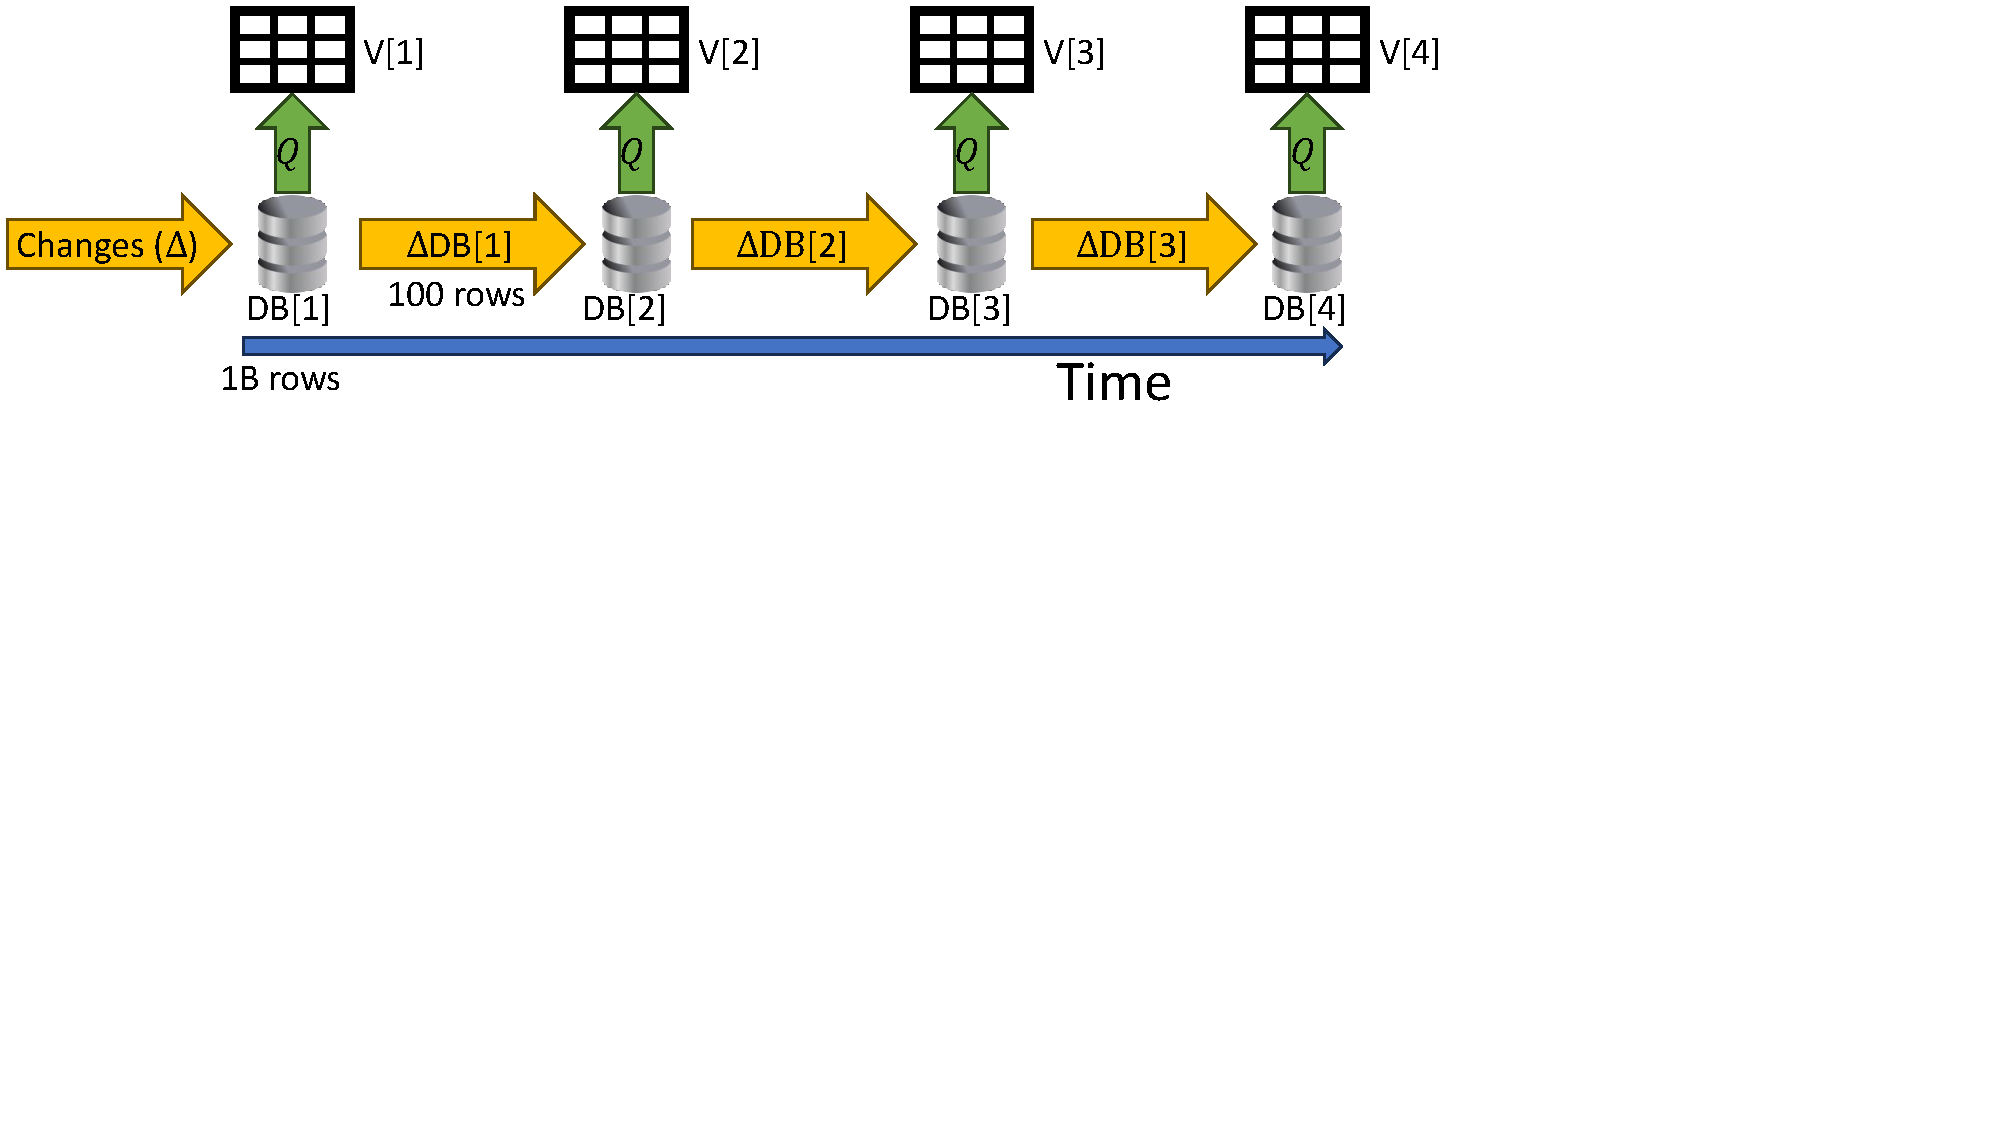
\includegraphics[trim={0 4.8in 3.7in 0},clip,scale=.30]{view.pdf}

The naive solution is expensive.  After the first version of the view
has been constructed, an ideal algorithm would compute only
\emph{changes} to the view $\Delta V$ doing work $O(|\Delta DB|)$.
Ideally, we want to construct a new query $\inc{Q}$ with the property
that $\Delta V = \inc{Q}(\Delta DB)$, i.e., $\inc{Q}$ can compute the
change of the view from the change of the database:

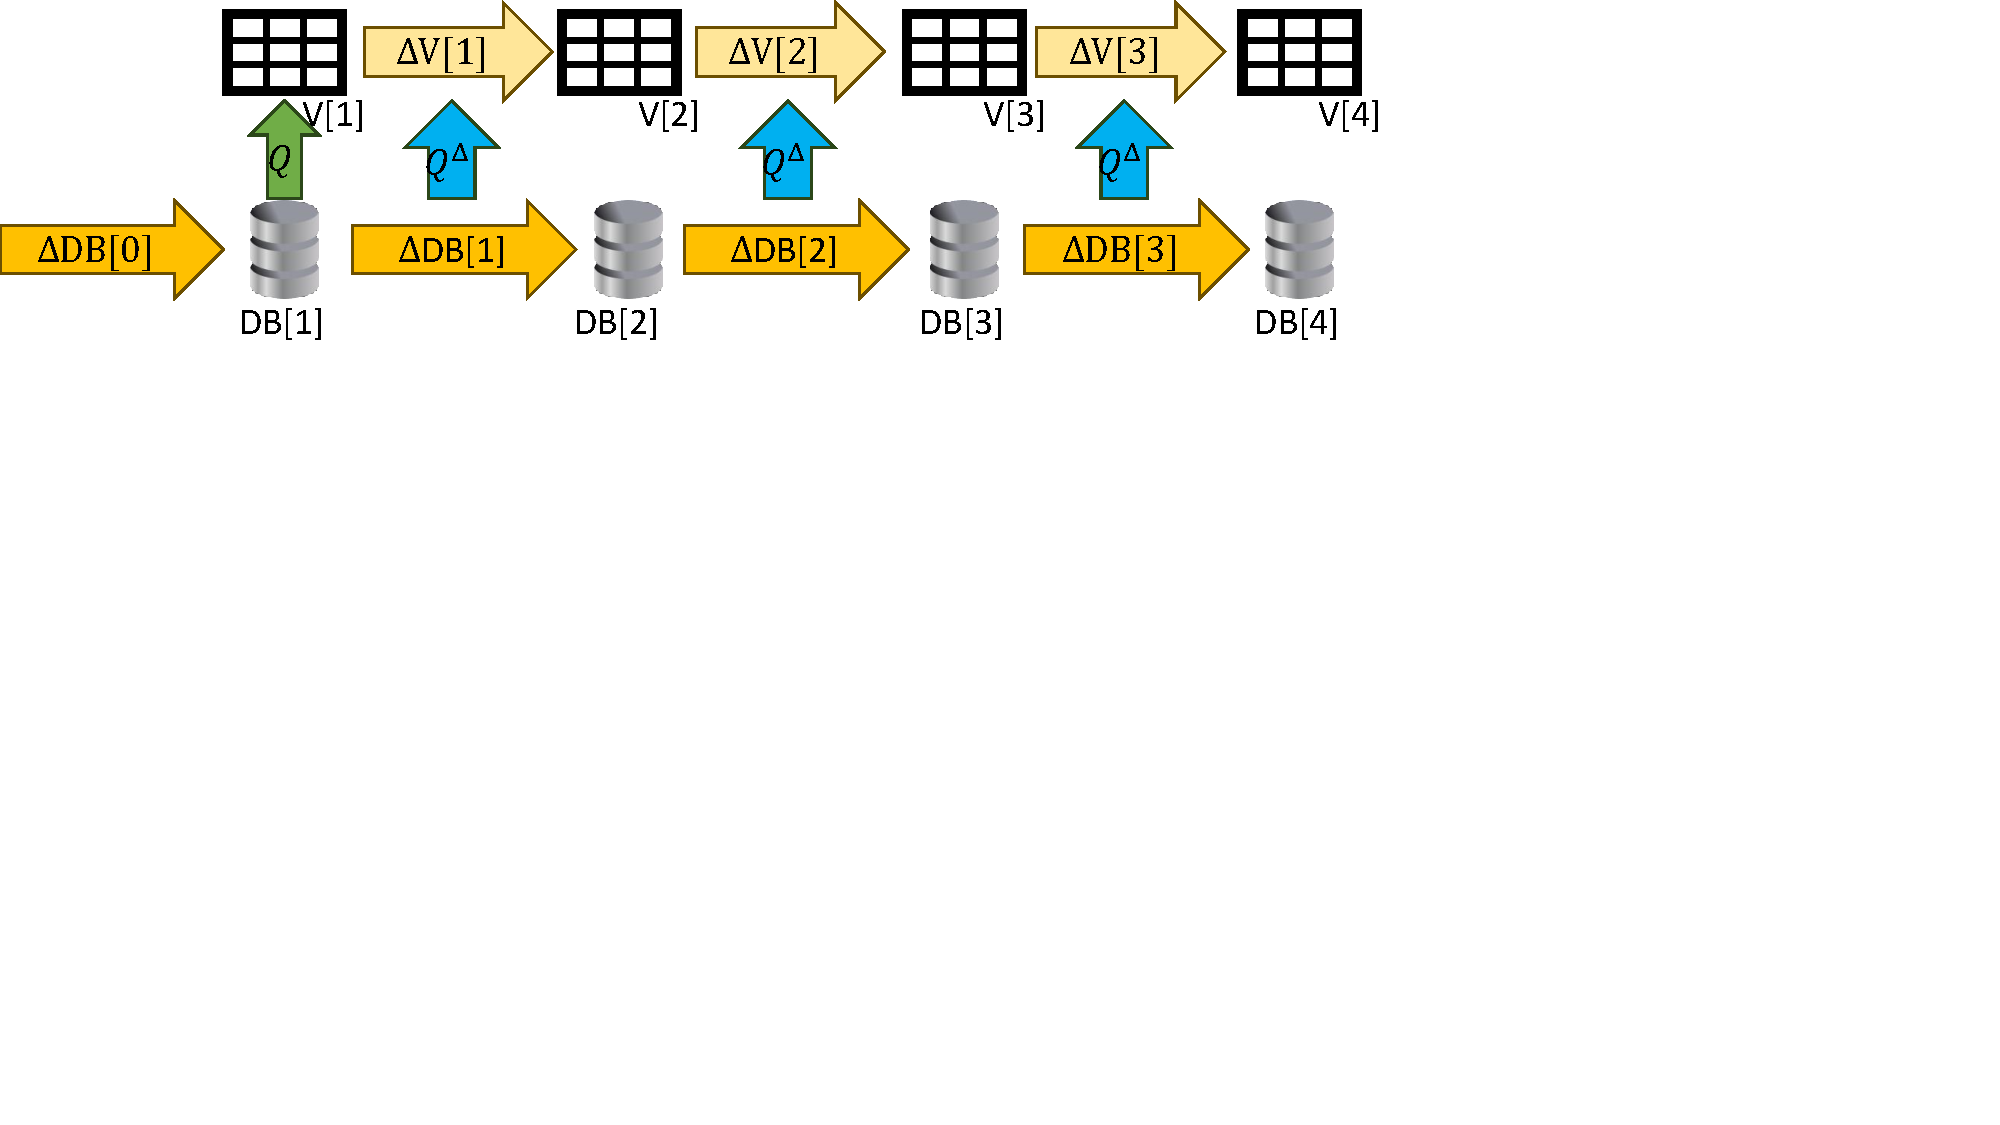
\includegraphics[trim={0 5.2in 4.1in 0},clip,scale=.30]{incview.pdf}

We call $\inc{Q}$ the \emph{incremental} version of $Q$.  If one
thinks of $\inc{Q}$ as a function of $\Delta DB$, one can show that
the ideal solution as described above is impossible to reach.

In this paper we propose a new way to define $\inc{Q}$, as a form of
\emph{computation on streams}.  Our model is inspired by Digital
Signal Processing DSP~\cite{rabiner-book75}, applied to databases,
hence the name \dbsp.  $\inc{Q}$ can be very efficient.  As for
traditional database queries, the performance of $\inc{Q}$ depends
both on the query $Q$ but also on the actual data that the query is
applied to.  Informally, $\inc{Q}$ built by our algorithm, is faster
than $Q$ by a factor of $O(|DB| / |\Delta DB|)$.  In practice this may
be an improvement of several orders of magnitude.  For our example
above $|DB| \approx 10^9$ and $|\Delta DB| \approx 10^2$, this can
make $\inc{Q}$ \textbf{10 million times} faster!

Instead of treating the database as a large changing object, we model
it as a \emph{sequence} or \emph{stream} of database snapshots.
Similarly, consecutive view snapshots form a stream.  \dbsp is a
simple programming language computing on \\streams; inputs and outputs
are streams of arbitrary values.

%Whereas previous IVM solutions are based on defining a notion of a
%(partial) derivative of $Q$ with respect to its inputs, our definition
%only requires computing \emph{derivatives of streams} as functions of
%time.  Derivatives of streams are always well-defined if the data
%computed on has a notion of difference that satisfies some simple
%mathematical properties --- specifically, that it forms a commutative
%group.  (Fortunately, relational databases can be modeled in such a
%way~\cite{green-pods07, koch-pods10}.)

The \dbsp language has only 4 operators.  However, it can express a
rich set of computations on streams, including repeated computations
(similar to the repeated queries $Q$ above), recursive computations
that compute fixed points (like Datalog programs), streaming
computations, and incremental computations (which we define shortly).
The full paper~\cite{budiu-vldb23} gives a precise mathematical
description of \dbsp, this presentation is simplified to convey the
main intuitions.  We omit the related work section from this
presentation.

The central result of this paper is Algorithm~\ref{algorithm-inc}
which, given a \dbsp program that computes on a stream of values,
mechanically transforms it into an incremental \dbsp program that
computes on a stream of changes.

\dbsp is not tied to databases in any way; it is in fact a
Turing-complete language that can be used for many other purposes.
But it works particularly well in the area of databases, for two
reasons:

\begin{itemize}[nosep, leftmargin=0pt, itemindent=0.5cm]
  \item \dbsp operates on values from a commutative group.  Databases
    can be modeled as a commutative group.
  \item \dbsp reduces the problem of incrementalizing a complex
    program to the problem of incrementalizing each primitive
    operation that appears in the program.  For databases there are
    known efficient incremental implementations for all primitive
    operations.
\end{itemize}

%\dbsp has several attractive properties:
%
%\begin{enumerate}
%\item it is \textbf{simple}.  \dbsp has only 4 operators, and it is
%  built entirely on elementary concepts such as functions and
%  algebraic groups.
%\item it is \textbf{expressive}.  It can be used to define precisely
%  multiple concepts: traditional queries, streaming computations, and
%  incremental computations.
%\item mathematically \textbf{precise}.  All the results in this paper
%  have been formalized and checked using the Lean proof
%  assistant~\cite{moura-cade15}.
%\item it is \textbf{modular}, in the following two ways:
%(a) the incremental version of a complex query can be reduced
%recursively to incrementalizing its component subqueries.
%This gives a simple, syntactic,
%heuristic-free algorithm (Algorithm~\ref{algorithm-inc})
%that converts an arbitrary \dbsp query plan to its incremental form.
%(b) Extending \dbsp to support new primitive operators is easy,
%and they immediately benefit from the rest of the theory of
%incrementalization.
%An important consequence of modularity is that the theory
%can be efficiently implemented, as we
%briefly discuss in \refsec{sec:implementation}.
%\end{enumerate}

\subsection{Circuits and Streams}\label{sec:intro-circuits}

In this paper we use circuit diagrams to depict programs.  In a
circuit a rectangle represents a function, and an arrow represents an
input or output value.  The following diagram shows a function $f$
consuming two inputs $i$ (input 0) and $j$ (input 1) and producing one
output $o = f(i, j)$:
%
\begin{center}
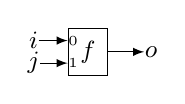
\begin{tikzpicture}[auto,>=latex,inner sep=0mm]
  \node[block, minimum height=.6cm, minimum width=.5cm] (function) {$f$};
  \node[below=1mm of function.north west,font=\tiny,anchor=north west] (0) {0};
  \node[above=1mm of function.south west,font=\tiny,anchor=south west] (1) {1};
  \node[left of=0, node distance=.5cm] (input0) {$i$};
  \node[left of=1, node distance=.5cm] (input1) {$j$};
  \node[right of=function, node distance=.8cm] (output) {$o$};
  \draw[->] (input0) -- (0);
  \draw[->] (input1) -- (1);
  \draw[->] (function) -- (output);
\end{tikzpicture}
\end{center}
\vspace{-1.2ex}
%
Most of the functions we deal with are commutative, so we can skip
inputs label, displaying the circuit above as:
%
\begin{center}
  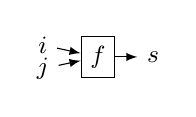
\begin{tikzpicture}[auto,>=latex, node distance=.7cm]
    \node[] (input0) {$i$};
    \node[below of=input0,node distance=.15cm] (dummy) {};
    \node[below of=dummy,node distance=.15cm] (input1) {$j$};
    \node[block, right of=dummy] (T) {$f$};
    \node[right of=T] (output) {$s$};
    \draw[->] (input0) -- (T);
    \draw[->] (input1) -- (T);
    \draw[->] (T) -- (output);
  \end{tikzpicture}
\end{center}
\vspace{-1.2ex}
%
Functions, and their circuits, can be composed, as in the following
example for the function $o = g(s) + (f(s) \times s)$:
%
\begin{center}
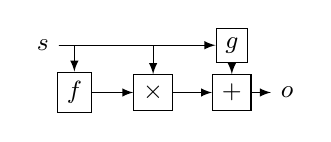
\begin{tikzpicture}[auto,>=latex]
  \node[] (input) {$s$};
  \node[] [right of=input, node distance=.4cm] (dummy) {};
  \node[block, below of=dummy, node distance=.6cm] (S1) {$f$};
  \node[block, right of=S1] (T1) {$\times$};
  \node[block, right of=T1] (T2) {$+$};
  \node[block, above of=T2, node distance=.6cm] (S2) {$g$};
  \node[right of=T2, node distance=.7cm] (output) {$o$};
  \draw[->] (input) -| (S1);
  \draw[->] (input) -| (T1);
  \draw[->] (S1) -- (T1);
  \draw[->] (T1) -- (T2);
  \draw[->] (input) -- (S2);
  \draw[->] (T2) -- (output);
  \draw[->] (S2) -- (T2);
\end{tikzpicture}
\end{center}
\vspace{-1ex}
%
We say that two circuits are \defined{equivalent} if they compute the
same function.  We use the symbol $\cong$ to indicate circuit
equivalence.  For example, we have the following circuit equivalence
(where $\circ$ is function composition):

\noindent
\begin{tabular}{m{3cm}m{.3cm}m{3cm}c}
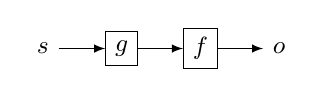
\begin{tikzpicture}[auto,>=latex]
  \node[] (input) {$s$};
  \node[block, right of=input] (g) {$g$};
  \node[block, right of=g] (f) {$f$};
  \node[right of=f] (output) {$o$};
  \draw[->] (input) -- (g);
  \draw[->] (g) -- (f);
  \draw[->] (f) -- (output);
\end{tikzpicture}
&
$\cong$
&
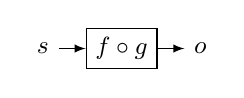
\begin{tikzpicture}[auto,>=latex]
    \node[] (input) {$s$};
    \node[block, right of=input, node distance=1cm] (fg) {$f \circ g$};
    \node[right of=fg, node distance=1cm] (output) {$o$};
    \draw[->] (input) -- (fg);
    \draw[->] (fg) -- (output);
\end{tikzpicture}
&
(*)
\end{tabular}
\vspace{-2ex}

\subsection{Streams}

The core notion of \dbsp is the \textbf{stream}.  Given a set $A$, a
\defined{stream} \emph{of values from $A$} is an infinite sequence of
values from $A$.  $\stream{A}$ denotes the set of all streams with
values from $A$.  We write $s[t]$ for the $t$-th element of the stream
$s$.  Think of $t$ as the ``time'' and of $s[t]\in A$ as the value of
the stream $s$ ``at time'' $t$.  We show streams as a sequence of
boxes, with time from \emph{right to left}: e.g., the stream $s[t] =
t$ is:
%
\begin{center}
\begin{tabular}{cc}
  \sv{0 1 2 3 4} \\
  $\xleftarrow[\hspace{1cm}\mathrm{time}\hspace{1cm}]{}$
\end{tabular}
\end{center}
\vspace{-1ex}
%
%\begin{definition}[stream operator]
A \defined{stream operator} is a function that computes on streams and
produces streams.
%\end{definition}
In general we use ``operator'' for streams, and ``function'' for
computations on ``scalar'' values.

We use arrows with a double head to depict streams.  The following
diagram shows a stream operator $T$ consuming two input streams $s_0$
and $s_1$, producing one output stream $s$:
%
\begin{center}
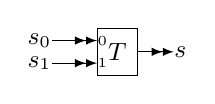
\begin{tikzpicture}[auto,>=latex,inner sep=0mm]
  \node[block, minimum height=.6cm, minimum width=.5cm] (function) {$T$};
  \node[below=1mm of function.north west,font=\tiny,anchor=north west] (0) {0};
  \node[above=1mm of function.south west,font=\tiny,anchor=south west] (1) {1};
  \node[left of=0, node distance=0.8cm] (input0) {$s_0$};
  \node[left of=1, node distance=0.8cm] (input1) {$s_1$};
  \node[right of=function, node distance=.8cm] (output) {$s$};
  \draw[->>] (input0) -- (0);
  \draw[->>] (input1) -- (1);
  \draw[->>] (function) -- (output);
\end{tikzpicture}
\vspace{-1ex}
\end{center}
%
We write $s = T(s_0, s_1)$.
%\begin{definition}(lifting)
Given a function $f: A \to B$, we define a stream operator $\lift{f}
:\stream{A} \to \stream{B}$ (read as ``$f$ lifted'') by applying
function $f$ to each input value independently:
\begin{center}
  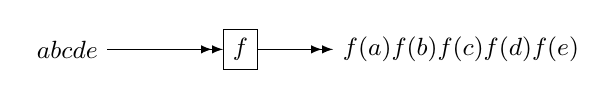
\begin{tikzpicture}[auto,>=latex]
    \node[] (input) {$\sv{a b c d e}$};
    \node[block, right of=input, node distance=2.2cm] (f) {$\lift{f}$};
    \node[right of=f, node distance=2.8cm] (output) {$\sv{f(a) f(b) f(c) f(d) f(e)}$};
    \draw[->>] (input) -- (f);
    \draw[->>] (f) -- (output);
  \end{tikzpicture}
\end{center}
\vspace{-1ex}
%\end{definition}

To simplify the notation, we write $a + b$ for streams $a, b$ instead
of $a (\lift{+}) b$; we also write $-a$ instead of $(\lift{-})a$.

\subsection{Databases as streams}

We generally think of streams as sequences of ``small'' values, such
as insertions or deletions in a database.  However, we also treat the
whole database as a \emph{stream of database snapshots}.  We model a
database as a stream $DB$.  Time is not wall-clock time, but counts
the transactions applied to the database.  Since transactions are
linearizable, they have a total order.  $DB[t]$ is the snapshot of the
database contents after $t$ transactions have been applied.  This
notation is apparent in the diagrams in \refsec{sec:intro-incremental}.

Database transactions also form a stream $\Delta DB$, this time a
stream of \emph{changes}, or \emph{deltas}, that are applied to the
database.  The values of this stream are defined by $(\Delta DB)[t] =
DB[t] - DB[t-1]$, where ``$-$'' stands for the difference between two
databases, a notion that we will soon make more precise.  The $\Delta
DB$ stream can be produced from the $DB$ stream by the \emph{stream
differentiation} operator $\D$; this operator produces as its output
the stream of changes from its input stream; we have thus $\D(DB) =
\Delta DB$.

Conversely, the database snapshot at time $t$ is the cumulative result
of applying all transactions up to $t$: $DB[t] = \Delta DB[0] + \Delta
DB[1] + \ldots + \Delta DB[t]$.  The stream operator $\I$ is defined
to produce each output by adding up all previous inputs.  We call $\I$
\emph{stream integration}, the inverse of differentiation.  The
following diagram shows the relationship between the streams $\Delta
DB$ and $DB$:
\begin{center}

\begin{tikzpicture}[auto,>=latex,minimum width=.5cm, node distance=1.2cm]
  \node[] (input) {$\Delta DB$};
  \node[block, right of=input] (I) {$\I$};
  \node[right of=I] (output) {$DB$};
  \node[block, right of=output] (D) {$\D$};
  \node[right of=D] (end) {$\Delta DB$};
  \draw[->>] (input) -- (I);
  \draw[->>] (I) -- (output);
  \draw[->>] (output) -- (D);
  \draw[->>] (D) -- (end);
\end{tikzpicture}
\end{center}

A view in this model is also a stream.  Suppose query $Q$ defining a
view $V$.  For each snapshot of the database stream we have a snapshot
of the view: $V[t] = Q(DB[t])$.  A view is thus just a lifted query:
$V = (\lift{Q})(DB)$.

Armed with these basic definitions, we can precisely define IVM.  What
does it mean to maintain a view incrementally?  A maintenance
algorithm needs to compute the \emph{changes} to the view given the
changes to the database. Given a query $Q$, a key contribution of this
paper is the definition of its \emph{incremental version} $\inc{Q}$,
using stream integration and differentiation, depicted graphically as:
\vspace{-2ex}
%
\begin{center}
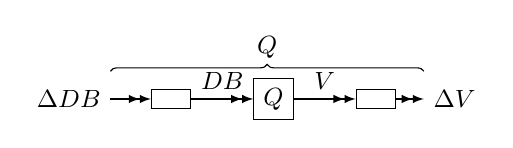
\begin{tikzpicture}[auto,>=latex,minimum width=.5cm]
  \node[] (input) {$\Delta DB$};
  \node[block, right of=input, node distance=1.3cm] (I) {$\I$};
  \node[block, right of=I, node distance=1.3cm] (Q) {$\lift{Q}$};
  \node[block, right of=Q, node distance=1.3cm] (D) {$\D$};
  \node[right of=D] (output) {$\Delta V$};
  \draw[->>] (input) -- (I);
  \draw[->>] (I) -- node (db) {$DB$} (Q);
  \draw[->>] (Q) -- node (B) {$V$} (D);
  \draw[->>] (D) -- (output);
  \draw[decorate, decoration = {brace, raise=10pt}] (input) -- (output)
  node[pos=.5, above=11pt]{$\inc{Q}$};
\end{tikzpicture}
\end{center}
\vspace{-1ex}
%
Mathematically: $\inc{Q} = \D \circ (\lift{Q}) \circ \I$.  The
incremental version of a query $Q$ is a \emph{streaming operator}
$\inc{Q}$ which computes directly on changes and produces changes.
The incremental version of a query is thus always well-defined.  The
above definition gives us one way to compute a query incrementally,
but applying it naively produces an inefficient execution, since it
reconstructs the database at each step.  It is in fact as bad as the
naive solution.  In \refsec{sec:incremental} we show how we can
optimize the implementation of $\inc{Q}$. The key property is that the
we can ``push'' the $\inc{.}$ operator ``down'' in a query plan:
$\inc{(Q_1 \circ Q_2)} = \inc{Q_1} \circ \inc{Q_2}$.

Armed with this general theory of incremental computation, in
\secref{sec:relational} we show how to model relational queries in
\dbsp.  This immediately gives us a general algorithm to compute the
incremental version of any relational query.  These results were
previously known, but they are cleanly modeled by \dbsp.
\secref{sec:recursion} shows how programs containing recursion can be
implemented and incrementalized in \dbsp.  For example, given an
implementation of transitive closure in the natural recursive way, our
algorithm produces a program that efficiently maintains the transitive
closure of a graph as nodes and edges are added and deleted.

\subsection{Contributions}

This work makes the following contributions:
\begin{enumerate}[nosep, leftmargin=0pt, itemindent=0.5cm, label=\textbf{(\arabic{*})}]
  \item We introduce \dbsp, a simple but expressive language for
    streaming computation. \dbsp gives an elegant formal foundation
    unifying the manipulation of streaming and incremental
    computations.
  \item An algorithm for incrementalizing any streaming computation
    expressed in \dbsp that handles arbitrary insertions and deletions
    from any of the data sources.
  \item An illustration of how \dbsp can model various classes of
    practical queries, such as relational algebra, nested relations,
    aggregations, and Datalog.
  \item The first general and machine-checked theory of IVM.  All the
    theoretical results in the original version of this
    paper~\cite{budiu-vldb23} have been checked~\cite{dbsp-theory}
    using the Lean proof assistant~\cite{moura-cade15}.
  \item A practical open-source implementation of this theory as a
    runtime and a SQL compiler.
\end{enumerate}


\section{Stream operators}\label{sec:streams}

%\subsection{Useful stream operators}\label{sec:abelian}

For the rest of this paper we require the set of values $A$ of a
stream $\stream{A}$ to form a commutative group, with operations $+$,
$-$, and a $0$ (zero) value.  The \emph{plus} defines what it means to
\emph{add} new data, while the \emph{minus} allows us to compute
differences (deltas).  We show later that this requirement is not a
problem for using \dbsp in the context of databases.

Stream operators are very powerful mathematically, but in \dbsp we
restrict ourselves to a very small subset.  All \dbsp computations are
\emph{causal}~\cite{causal}: the output at time $t$ is produced
immediately after all inputs up at time $t$ have been received; the
output at time $t$ cannot depend on inputs arriving after $t$.

The following circuit equivalence tells us that we can lift a circuit
by lifting each of its functions separately:

\noindent
\begin{tabular}{m{3cm}m{.3cm}m{3cm}c}
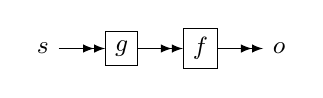
\begin{tikzpicture}[auto,>=latex]
  \node[] (input) {$s$};
  \node[block, right of=input] (g) {$\lift{g}$};
  \node[block, right of=g] (f) {$\lift{f}$};
  \node[right of=f] (output) {$o$};
  \draw[->>] (input) -- (g);
  \draw[->>] (g) -- (f);
  \draw[->>] (f) -- (output);
\end{tikzpicture}
&
$\cong$
&
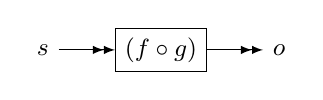
\begin{tikzpicture}[auto,>=latex]
    \node[] (input) {$s$};
    \node[block, right of=input, node distance=1.5cm] (fg) {$\lift{(f \circ g)}$};
    \node[right of=fg, node distance=1.5cm] (output) {$o$};
    \draw[->>] (input) -- (fg);
    \draw[->>] (fg) -- (output);
\end{tikzpicture}
&
(**)
\end{tabular}


%\subsubsection{Delays}\label{sec:delay}

%\begin{definition}[Delay]
The \defined{delay operator} $z^{-1}$ produces an output stream by
delaying its input by one step (and starting with a
zero)\footnote{This bizarre name comes from digital signal
processing.}:
%
\begin{center}
  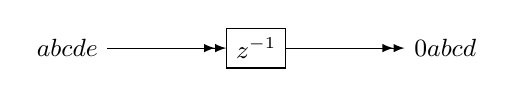
\begin{tikzpicture}[auto,>=latex,node distance=2.4cm]
    \node[] (input) {$\sv{a b c d e}$};
    \node[block, right of=input] (z) {$z^{-1}$};
    \node[right of=z] (output) {$\sv{0 a b c d}$};
    \draw[->>] (input) -- (z);
    \draw[->>] (z) -- (output);
  \end{tikzpicture}
\end{center}
\vspace{-1ex}
%\end{definition}
%
A very important property of the delay operator is that it produces
the first output \emph{before} having received the first input, and it
produces the second output before having received the second input,
etc.

%\begin{definition}[Time invariance]
%A stream operator $S: \stream{A} \to \stream{B}$ is \defined{time-invariant} (TI) if
%$S(\zm_A(s)) = \zm_B(S(s))$ for all $s \in \stream{A}$; in other words, if
%the following two circuits are equivalent:
%
%\begin{tabular}{m{3cm}m{.5cm}m{3cm}}
%\begin{tikzpicture}[auto,>=latex]
%  \node[] (input) {$s$};
%  \node[block, right of=input] (S) {$S$};
%  \node[block, right of=S] (z) {$\zm$};
%  \node[right of=z] (output) {$o$};
%  \draw[->] (input) -- (S);
%  \draw[->] (S) -- (z);
%  \draw[->] (z) -- (output);
%\end{tikzpicture}
%&
%$\cong$
%&
%\begin{tikzpicture}[auto,>=latex]
%  \node[] (input) {$s$};
%  \node[block, right of=input] (z) {$\zm$};
%  \node[block, right of=z] (S) {$S$};
%  \node[right of=S] (output) {$o$};
%  \draw[->] (input) -- (z);
%  \draw[->] (z) -- (S);
%  \draw[->] (S) -- (output);
%\end{tikzpicture}
%\end{tabular}
%
%\noindent
%This definition extends
%naturally to operators with multiple inputs.
%\end{definition}
%
%The composition of TI operators of any number of inputs
%is TI. The delay operator $\zm$ is TI.
%\dbsp only uses TI operators.
%
%%\begin{definition}
%%We say that a function between groups $f: A \to B$ has the \emph{zero-preservation
%%property} if $f(0_A) = 0_B$.  We write $\zpp{f}$.
%%\end{definition}
%%
%%A lifted operator $\lift{f}$ is TI iff $\zpp{f}$.
%
%\subsubsection{Causal and strict operators}\label{sec:causal}
%
%\begin{definition}[Causality]
%A stream operator $S:\stream{A}\to\stream{B}$
%is \defined{causal} when for all $s,s'\in\stream{A}$,
%and all times $t$ we have:
%$
%(\forall i \leq t . s[i]=s'[i]) ~~\Rightarrow~~ S(s)[t]=S(s')[t].
%$
%\end{definition}
%
%\noindent
%In other words, the output value at time $t$ can only depend on
%input values from times $t' \leq t$.
%Operators produced by lifting are causal, and $\zm$ is causal.
%All \dbsp operators are causal.  The composition
%of causal operators of any number of inputs is causal.
%
%\begin{definition}[Strictness]
%A stream operator, $F:\stream{A}\to\stream{B}$
%is \defined{strict}
%if  $\forall s,s'\in\stream{A}, \forall t \in \N$ we have:
%$(\forall i<t . ~s[i]=s'[i]) ~~\Rightarrow \\ F(s)[t]=F(s')[t].$
%\end{definition}
%
%In other words, the $t$-th output of $F(s)$ can depend only on ``past'' values
%of the input $s$, between $0$ and $t-1$.
%In particular, $F(s)[0] = 0_B$ is the same for all $s \in \stream{A}$.
%Strict operators are causal. Lifted operators in general are \emph{not} strict.
%$\zm$ is strict.  %In \dbsp $\zm$ is the only primitive strict operator.
%
%\begin{proposition}
%\label{prop-unique-fix}
%For a strict $F: \stream{A} \to \stream{A}$ the equation ~$\alpha=F(\alpha)$~ has a unique
%solution $\alpha \in \stream{A}$, denoted by $\fix{\alpha}{F(\alpha)}$.
%\end{proposition}
%
%Thus every strict operator from a set to itself has a unique fixed
%point.  The simple proof relies on strong induction, showing that the
%solution $\alpha[t]$ depends only on the values of $\alpha$ prior to
%$t$.
%
%Consider a circuit with a strict feedback edge:
%\begin{center}
%\begin{tikzpicture}[>=latex]
%    \node[] (input) {$s$};
%    \node[block, right of=input] (f) {$T$};
%    \node[right of=f] (output) {$\alpha$};
%    \node[block, below of=f, node distance=.5cm] (z) {$F$};
%    \draw[->] (input) -- (f);
%    \draw[->] (f) -- node (mid) {} (output);
%    \draw[->] (mid.center) |-  (z);
%    \draw[->] (z.west) -- ++(-.3,0) |- ([yshift=1mm]f.south west);
%\end{tikzpicture}
%\end{center}
%
%This circuit is a well-defined function on streams:
%
%%\begin{lemma}
%%\label{lemma-causal-strict}
%%If $F: \stream{B} \to \stream{B}$ is strict and $T: \stream{A} \times \stream{B} \to \stream{B}$ is causal, then for fixed $s$ the operator
%%$\lambda\alpha.T(s,F(\alpha)): \stream{A} \to \stream{B}$ is strict.
%%\end{lemma}
%
%\begin{lemma}\label{feedback-semantics}
%\label{cor-loop}
%If $F: \stream{B} \to \stream{B}$ is strict and $T: \stream{A} \times \stream{B} \to \stream{B}$ is causal,
%the operator $Q(s)=\fix{\alpha}{T(s,F(\alpha))}$ is well-defined and causal.
%If, moreover, $F$ and $T$ are TI then so is $Q$.
%\end{lemma}
%
%All \dbsp computations are built using just lifted functions and
%delays.  We add two more operators in \secref{sec:nested}.
%
%\subsection{Integration and differentiation}\label{sec:abelianstreams}

%Remember that we require the elements of a stream to come from an abelian group $A$.
%Streams themselves form an abelian group:
%
%\begin{proposition}
%The structure $(\stream{A},+,0,-)$, obtained by lifting the $+$ and unary $-$ operations of $A$,
%is an abelian group.  0 is the stream with all values $0_A$.
%\end{proposition}
%
%\noindent
%Stream addition and negation are causal, TI operators.

%Given a linear function $f: A \to B$, the stream operator $\lift{f}$
%is linear and TI (LTI).  $\zm$ is also LTI.
%
%\begin{definition}(bilinear)
%A function of two arguments $f: A \times B \to C$ with $A, B, C$ groups, is \emph{bilinear}
%if it is linear separately in each argument (i.e., it distributes over addition):
%$\forall a, b, c, d . f(a+b, c) = f(a, c) + f(b, c)$, and $f(a, c+d) = f(a, c) + f(c, d).$
%\end{definition}
%
%This definition extends to stream operators.
%The lifting of a bilinear function $f$ is
%a bilinear stream operator $\lift{f}$.  An example
%is lifted multiplication:
%$f: \stream{\N} \times \stream{\N} \to \stream{\N}, f(a, b)[t] = a[t]\cdot b[t]$.

%The composition of (bi)linear operators with linear operators
%is (bi)linear (since homomorphisms compose).

%The ``feedback loop'' of a linear operator is linear:
%
%\begin{proposition}
%\label{prop-rec-linear}
%Let $S$ be a unary, causal, LTI operator. The
%operator $Q(s)=\fix{\alpha}{S(s+\zm(\alpha))}$ is well-defined and LTI:
%
%\begin{center}
%\begin{tikzpicture}[>=latex]
%    \node[] (input) {$s$};
%    \node[block, shape=circle, right of=input, inner sep=0pt, node distance=.6cm] (plus) {$+$};
%    \node[block, right of=plus, node distance=.6cm] (Q) {$S$};
%    \node[right of=Q, node distance=1.2cm] (output) {$\alpha$};
%    \node[block, below of=Q, node distance=.6cm] (z) {$\zm$};
%    \draw[->] (input) -- (plus);
%    \draw[->] (plus) -- (Q);
%    \draw[->] (Q) -- node (mid) {} (output);
%    \draw[->] (mid.center) |-  (z);
%    \draw[->] (z) -| (plus);
%\end{tikzpicture}
%\end{center}
%\end{proposition}

%\begin{definition}[Differentiation]
We define the \defined{differentiation operator} as a composition of
several other operators: $\D(s) \defn s - \zm(s)$, shown as:
%
\vspace{-2ex}
\begin{center}
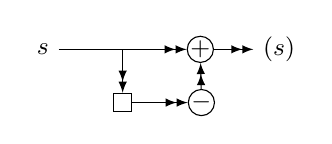
\begin{tikzpicture}[auto,>=latex,node distance=1cm]
    \node[] (input) {$s$};
    \node[block, shape=circle, right of=input, inner sep=0pt,node distance=2cm] (plus) {$+$};
    \node[right of=plus] (output) {$\D(s)$};
    \draw[->>] (input) -- node (i) {} (plus);
    \node[block, below of=i, node distance=.8cm] (z) {$\zm$};
    \node[block, shape=circle, right of=z, inner sep=0pt] (minus) {$-$};
    \draw[->>] (plus) -- (output);
    \draw[->>] (i) -- (z);
    \draw[->>] (z) -- (minus);
    \draw[->>] (minus) -- (plus);
\end{tikzpicture}
\end{center}
%\end{definition}
%We generally omit the type, and write just $\D$.
%The value of $\D(s)[t] = s[t] - s[t-1]$ if $t > 0$.
%
If $s$ is a stream, then $\D(s)$ is the \emph{stream of changes} of
$s$; a value in the output is the difference between two consecutive
values in the input.  As an example:
{
\noindent \small
\begin{align*}
  &\D(\sv{0 1 2 1 0}) &= \\
  &\sv{0 1 2 1 0} - \zm(\sv{0 1 2 1 0}) &=\\
  &\sv{0 1 2 1 0} - \sv{0 0 1 2 1} &=\\
%  &\sv{0-0 1-0 2-1 1-2 0-1} =\\
  &\sv{0 1 1 -1 -1}
\end{align*}
}

%\begin{proposition}
%\label{prop-diff-properties}
%$\D$ is causal and LTI.
%\end{proposition}

%The integration operator ``reconstitutes'' a stream from its changes:

%\begin{definition}[Integration]
The \defined{integration operator}
is given by the following circuit:
\vspace{-2ex}
\begin{center}
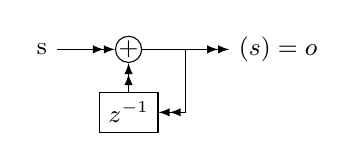
\begin{tikzpicture}[auto,>=latex, node distance=1.1cm]
    \node[] (input) {s};
    \node[block, shape=circle, right of=input, inner sep=0pt] (plus) {$+$};
    \node[right of=plus, node distance=1.9cm] (output) {$\I(s) = o$};
    \node[block, below of=plus, node distance=.8cm] (z) {$z^{-1}$};
    \draw[->>] (input) -- (plus);
    \draw[->>] (plus) -- node (o) {} (output);
    \draw[->>] (o) |- (z);
    \draw[->>] (z) -- (plus);
\end{tikzpicture}
\end{center}
\vspace{-1ex}
%\end{definition}
%
While this definition may seem strange, because the output stream is
used to compute itself, the use of the delay in the ``feedback'' loop
ensures that only \emph{previous} values of the output are used in
computing the current one.  Using the notation $o = \I(s)$ to make
formulas more readable, we can see the contents of stream $o$ is
produced step by step:
\begin{align*}
  o[0] &= s[0] + (\zm(o))[0] = s[0] + 0 = s[0] \\
  o[1] &= s[1] + (\zm(o))[1] = s[1] + o[0] = s[1] + s[0] \\
  o[2] &= s[2] + (\zm(o))[2] = s[2] + o[1] = s[2] + (s[1] + s[0])
\end{align*}

%\noindent
%We also generally omit the type, and write just $\I$.
%This is the construction from Proposition~\ref{prop-rec-linear}
%using the identity function for $S$.
%
%\begin{proposition}
%$\I(s)$ is the discrete (indefinite) integral applied to the stream $s$:
%\end{proposition}
In general, $\I(s)[t] = o[t] = \sum_{i \leq t} s[i]$.
Examples:
\begin{align*}
  \I(\sv{0 1 2 3 4 5}) &= \sv{0 1 3 6 10} \\
  \I(\sv{0 1 1 -1 -1}) &= \sv{0 1 2 1 0}.
\end{align*}

%\begin{proposition}
%\label{prop-integ-properties}
%$\I$ is causal and LTI.
%\end{proposition}
%
%\begin{theorem}[Inversion]
%\label{inverses}
%Integration and differentiation are inverses of each other:
%$\forall s . \I(\D(s)) = \D(\I(s)) = s$.
%\end{theorem}

Integration and differentiation are inverses of each other: while $\D$
computes the changes of a stream, $\I$ reconstitutes the original
stream given the stream of changes.  $\I$ and $\D$ ``cancel out'' when
applied in sequence:

\noindent
\begin{tabular}{m{2.5cm}m{.3cm}m{1cm}m{.3cm}m{2.5cm}}
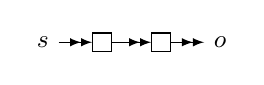
\begin{tikzpicture}[auto,>=latex, node distance=.75cm]
    \node[] (input) {$s$};
    \node[block, right of=input] (I) {$\I$};
    \node[block, right of=I] (D) {$\D$};
    \node[right of=D] (output) {$o$};
    \draw[->>] (input) -- (I);
    \draw[->>] (I) -- (D);
    \draw[->>] (D) -- (output);
\end{tikzpicture}
     &
     $\cong$
     &
     \hspace{-2ex}
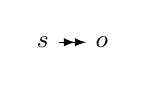
\begin{tikzpicture}[auto,>=latex, node distance=.75cm]
    \node[] (input) {$s$};
    \node[right of=input] (output) {$o$};
    \draw[->>] (input) -- (output);
\end{tikzpicture}
     &
     $\cong$
     &
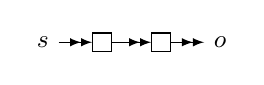
\begin{tikzpicture}[auto,>=latex, node distance=.75cm]
    \node[] (input) {$s$};
    \node[block, right of=input] (D) {$\D$};
    \node[block, right of=D] (I) {$\I$};
    \node[right of=I] (output) {$o$};
    \draw[->>] (input) -- (D);
    \draw[->>] (D) -- (I);
    \draw[->>] (I) -- (output);
\end{tikzpicture}
\end{tabular}

\section{Incremental view maintenance}\label{sec:incremental}

The results in this section are not specific to databases, they hold
for any stream computations, but we hint about their applicability for
databases.

%Here we define IVM and analyze its properties.

%\begin{definition}
Given a stream operator $S: \stream{A} \to \stream{B}$ we define the
\defined{incremental version} of $S$ as:
%\begin{equation}\label{def:inc}
%\inc{Q} \defn \D \circ Q \circ \I.
%\end{equation}
%$\inc{Q}$ has the same ``type'' as $Q$: $\inc{Q}: \stream{A} \to \stream{B}$.

%The following diagram illustrates the intuition behind this
%definition:
\vspace{-2ex}
\begin{center}
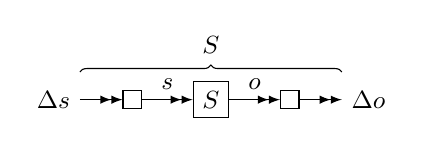
\begin{tikzpicture}[auto,>=latex]
    \node[] (input) {$\Delta s$};
    \node[block, right of=input] (I) {$\I$};
    \node[block, right of=I] (Q) {$S$};
    \node[block, right of=Q] (D) {$\D$};
    \node[right of=D] (output) {$\Delta o$};
    \draw[->>] (input) -- (I);
    \draw[->>] (I) -- node (s) {$s$} (Q);
    \draw[->>] (Q) -- node (o) {$o$} (D);
    \draw[->>] (D) -- (output);
    \draw[decorate, decoration = {brace, raise=10pt}] (input) -- (output)
    node[pos=.5, above=13pt]{$\inc{S}$};
\end{tikzpicture}
\end{center}
\vspace{-1ex}
%\end{definition}

If $S$ computes on a stream $s$, then $\inc{S}$ computes on a stream
of changes to $s$.  If $S$ produces a stream $o$, then $\inc{S}$
produces the stream of changes to $o$.  Note that this definition does
not require $S$ to be a lifted function.

For an operator with multiple inputs and outputs we define the
incremental version by applying $\I$ to each input, and $\D$ to each
output, e.g.: $\inc{T}(a, b) \defn \D (T(\I(a), \I(b)))$.

%Notice that our definition of incremental computation is meaningful only for \emph{streaming}
%computations; this is in contrast to classic definitions, e.g.~\cite{gupta-idb95} which
%consider only one change.  Generalizing the definition to operate on streams gives us
%additional power, especially when operating with recursive queries.
%
%The following proposition is one of our central results:
$\inc{S}$ has many nice properties:

%\begin{proposition}(Properties of the incremental version):
%\label{prop-inc-properties}
%\begin{description}
%\item[inversion:] $Q\mapsto\inc{Q}$ is bijective; its inverse is $Q\mapsto \I\circ Q\circ\D$.
%\item[invariance:] $\inc{+} = +, \inc{(\zm)} = \zm, \inc{-} = -, \inc{\I}=\I, \inc{\D}=\D$
%\item[push/pull:] \label{prop-part-commutation}
%    $Q \circ \I = \I \circ \inc{Q}$; $\D\circ Q = \inc{Q}\circ\D$
%\item[chain:] $\inc{(Q_1\circ Q_2)} = \inc{Q_1}\circ\inc{Q_2}$ (Generalizes to multiple inputs.)
%\item[add:] $\inc{(Q_1 + Q_2)} = \inc{Q_1} + \inc{Q_2}$
%\item[cycle:] $\inc{(\lambda s. \fix{\alpha}{T(s,\zm(\alpha)}))} = \lambda s. \fix{\alpha}{\inc{T}(s,\zm(\alpha)})$
%\end{description}
%\end{proposition}
%
The \defined{chain rule} states that $\inc{(Q_1 \circ Q_2)} =
\inc{Q_1} \circ \inc{Q_2}$, i.e., these circuits are equivalent:

\noindent
\begin{tabular}{cr}
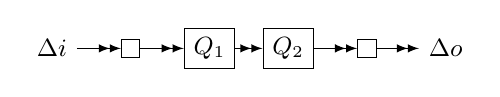
\begin{tikzpicture}[auto,>=latex]
  \node[] (input) {$\Delta i$};
  \node[block, right of=input] (I) {$\I$};
  \node[block, right of=I] (Q1) {$Q_1$};
  \node[block, right of=Q1] (Q2) {$Q_2$};
  \node[block, right of=Q2] (D) {$\D$};
  \node[right of=D] (output)  {$\Delta o$};
  \draw[->>] (input) -- (I);
  \draw[->>] (I) -- (Q1);
  \draw[->>] (Q1) -- (Q2);
  \draw[->>] (Q2) -- (D);
  \draw[->>] (D) -- (output);
\end{tikzpicture} &
$\cong$ \\
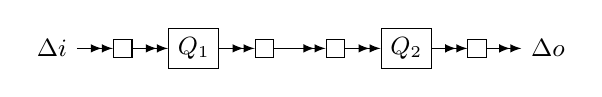
\begin{tikzpicture}[>=latex, node distance=.9cm]
  \node[] (input) {$\Delta i$};
  \node[block, right of=input] (I1) {$\I$};
  \node[block, right of=I1] (Q1) {$Q_1$};
  \node[block, right of=Q1] (D1) {$\D$};
  \node[block, right of=D1] (I2) {$\I$};
  \node[block, right of=I2] (Q2) {$Q_2$};
  \node[block, right of=Q2] (D2) {$\D$};
  \node[right of=D2] (output)  {$\Delta o$};
  \draw[->>] (input) -- (I1);
  \draw[->>] (I1) -- (Q1);
  \draw[->>] (Q1) -- (D1);
  \draw[->>] (D1) -- (I2);
  \draw[->>] (I2) -- (Q2);
  \draw[->>] (Q2) -- (D2);
  \draw[->>] (D2) -- (output);
\end{tikzpicture} &
$\cong$ \\
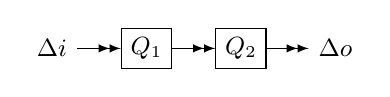
\begin{tikzpicture}[>=latex, node distance=1.2cm]
  \node[] (input) {$\Delta i$};
  \node[block, right of=input] (Q1) {$\inc{Q_1}$};
  \node[block, right of=Q1] (Q2) {$\inc{Q_2}$};
  \node[right of=Q2] (output)  {$\Delta o$};
  \draw[->>] (input) -- (Q1);
  \draw[->>] (Q1) -- (Q2);
  \draw[->>] (Q2) -- (output);
\end{tikzpicture}
\end{tabular}

\noindent In the database world, we can read this as: \textbf{to
  incrementalize a composite query you can incrementalize each
  sub-query independently}.  This gives us a simple deterministic
recipe reducing the incremental version of an arbitrary query to the
incremental version of its primitive operators.

The \defined{cycle rule} states that these circuits are equivalent:

\noindent
\begin{tabular}{m{4.4cm}m{.2cm}m{3cm}}
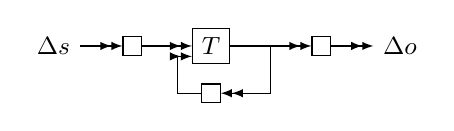
\begin{tikzpicture}[>=latex]
    \node[] (input) {$\Delta s$};
    \node[block, right of=input] (I) {$\I$};
    \node[block, right of=I] (f) {$T$};
    \node[block, right of=f, node distance=1.4cm] (D) {$\D$};
    \node[right of=D] (output) {$\Delta o$};
    \node[block, below of=f, node distance=.6cm] (z) {$\zm$};
    \draw[->>] (input) -- (I);
    \draw[->>] (I) -- (f);
    \draw[->>] (f) -- node (mid) {} (D);
    \draw[->>] (mid.center) |-  (z);
    \draw[->>] (z.west) -- ++(-.3,0) |- ([yshift=1mm]f.south west);
    \draw[->>] (D) -- (output);
\end{tikzpicture} & $\cong$ &
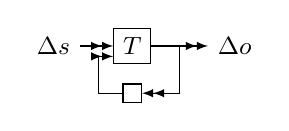
\begin{tikzpicture}[>=latex]
    \node[] (input) {$\Delta s$};
    \node[block, right of=input] (f) {$\inc{T}$};
    \node[right of=f, node distance=1.3cm] (output) {$\Delta o$};
    \node[block, below of=f, node distance=.6cm] (z) {$\zm$};
    \draw[->>] (input) -- (f);
    \draw[->>] (f) -- node (mid) {} (output);
    \draw[->>] (mid.center) |-  (z);
    \draw[->>] (z.west) -- ++(-.3,0) |- ([yshift=1mm]f.south west);
\end{tikzpicture}
\end{tabular}

\noindent
(We have omitted the labels on the inputs of $T$.) In other words, the
incremental version of a feedback loop around a query is just the
feedback loop with the incremental query for its body.  This result
will be useful for recursive queries.

%To execute incremental queries efficiently, we want to compute directly
%on streams of changes, without integrating them. The invariance property above shows
%that stream operators $+$, $-$, and $\zm$ are identical to their incremental versions.
%The following theorems generalize this to linear and bi-linear operators:

We call an operator $S$ \defined{linear} if it has the property that
$S(a+b) = S(a) + S(b)$ (where $+$ is the addition of streams).
%
%\begin{theorem}[Linear]\label{linear}
For a linear operator $S$ we have $\inc{S}=S$.
%\end{theorem}
%
This is very useful because many primitive database operations can be
implemented as linear operators: selection, projection, filtering,
grouping, parts of aggregation are all linear.  Moreover, the
following operators are linear: $-$, $z^{-1}$, $\I$, $\D$, $\lift{f}$
if $f$ is a linear function.

We call an operator $T$ with two inputs \defined{bilinear} if it
distributes over stream addition: $T(a+b, c) = T(a, c) + T(b, c)$, and
$T(a, c+d) = T(a, c) + T(a, d)$.  (Similar to multiplication's
distributivity over addition.)  In databases intersection, joins, and
Cartesian products are bilinear.

%\begin{theorem}[Bilinear]\label{bilinear}
Using infix notation, for a bilinear operator $\times$ we have:
\begin{eqnarray*}
\inc{(\Delta a \times \Delta b)} = \\
(\Delta a \times \Delta b ~+~ \zm(\I(\Delta a)) \times
\Delta b ~+~ \Delta a \times \zm(\I(\Delta b)) = \\
\Delta a \times \Delta b + \zm(a) \times \Delta b + \Delta a \times \zm(b)
\end{eqnarray*}

If we ignore the delay operators in this equation we recover the
well-known formula for join delta queries, e.g.,\cite{koch-pods10}.

%In pictures: \\
\noindent
\begin{tabular}{m{3.3cm}m{0cm}m{4cm}%m{0cm}m{2.8cm}
  }
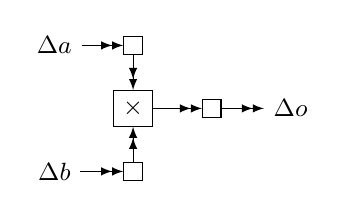
\begin{tikzpicture}[auto,>=latex]
    \node[] (a) {$\Delta a$};
    \node[block, right of=a] (ai) {$\I$};
    \node[below of=a, node distance=.8cm] (midway) {};
    \node[below of=midway, node distance=.8cm] (b) {$\Delta b$};
    \node[block, right of=b] (bi) {$\I$};
    \node[block, right of=midway, node distance=1cm] (q) {$\times$};
    \node[block, right of=q] (D) {$\D$};
    \node[right of=D] (output) {$\Delta o$};
    \draw[->>] (a) -- (ai);
    \draw[->>] (b) -- (bi);
    \draw[->>] (ai) -- (q);
    \draw[->>] (bi) -- (q);
    \draw[->>] (q) -- (D);
    \draw[->>] (D) -- (output);
\end{tikzpicture} &
$\cong$ &
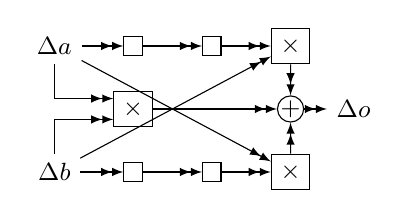
\begin{tikzpicture}[auto,>=latex]
  \node[] (input1) {$\Delta a$};
  \node[below of=input1, node distance=1.6cm] (input2) {$\Delta b$};
  \node[block, right of=input1, node distance=1cm] (I1) {$\I$};
  \node[block, below of=I1,node distance=.8cm] (ab) {$\times$};
  \node[block, right of=input2, node distance=1cm] (I2) {$\I$};
  \draw[->>] (input1) -- (I1);
  \draw[->>] (input2) -- (I2);
  \draw[->>] (input1) |- ([yshift=-1mm]ab.north west);
  \draw[->>] (input2) |- ([yshift=1mm]ab.south west);
  \node[block, right of=I1] (ZI1) {$\zm$};
  \node[block, right of=I2] (ZI2) {$\zm$};
  \draw[->>] (I1) -- (ZI1);
  \draw[->>] (I2) -- (ZI2);
  \node[block, right of=ZI1] (DI1) {$\times$};
  \node[block, right of=ZI2] (DI2) {$\times$};
  \draw[->>] (ZI1) -- (DI1);
  \draw[->>] (ZI2) -- (DI2);
  \node[block, circle, right of=ab, inner sep=0cm, node distance=2cm] (sum) {$+$};
  \draw[->>] (ab) -- (sum);
  \draw[->>] (DI1) -- (sum);
  \draw[->>] (DI2) -- (sum);
  \node[right of=sum, node distance=.8cm] (output) {$\Delta o$};
  \draw[->>] (sum) -- (output);
  \draw[->>] (input1) -- (DI2);
  \draw[->>] (input2) -- (DI1);
\end{tikzpicture}
%&
%$\cong$ &
%\begin{tikzpicture}[auto,>=latex,node distance=.7cm]
%  \node[] (input1) {$a$};
%  \node[below of=input1, node distance=1cm] (input2) {$b$};
%  \node[block, right of=input1, node distance=.5cm] (I1) {$\I$};
%  \node[block, right of=input2, node distance=.5cm] (I2) {$\I$};
%  \draw[->>] (input1) -- (I1);
%  \draw[->>] (input2) -- (I2);
%  \node[block, right of=I2] (ZI2) {$\zm$};
%  \draw[->>] (I2) -- (ZI2);
%  \node[block, right of=I1] (DI1) {$\times$};
%  \node[block, right of=ZI2] (DI2) {$\times$};
%  \draw[->>] (I1) -- (DI1);
%  \draw[->>] (ZI2) -- (DI2);
%  \node[block, circle, above of=DI2, inner sep=0cm, node distance=.5cm] (sum) {$+$};
%  \draw[->>] (DI1) -- (sum);
%  \draw[->>] (DI2) -- (sum);
%  \node[right of=sum, node distance=.5cm] (output) {$o$};
%  \draw[->>] (sum) -- (output);
%  \draw[->>] (input1) -- (DI2);
%  \draw[->>] (input2) -- (DI1);
%\end{tikzpicture}
\end{tabular}
%\end{theorem}

What is the intuition behind this diagram?  Let us consider the case
of Cartesian product $a \times b$.  The incremental product has inputs
$\Delta a = \D(a)$ and $\Delta b = \D(b)$.  What happens when we add a
row $x$ to relation $a$ (i.e., $\Delta a = x$)?  The new row $x$ will
appear in the output change combined with every row in the
\emph{previous version} of the \emph{full} relation $b$.  The operator
$\I(\Delta b)$ in fact computes relation $b$ from the stream $\Delta
b$ of changes, and $\zm$ applied to this value gives us its previous
version.  So the bottom $\times$ operator computes $x \times \zm(b) =
\Delta a \times \zm(\I(\Delta b))$, the change produced by the new row
$x$.  The top $\times$ operator performs the symmetric operation for
the changes of the $b$ relation.  The middle $\times$ operator
produces the results of changes to both inputs.

%Rewriting this statement using $\Delta a$ for the stream of changes to
%$a$ we get the familiar formula for incremental equi-joins:
%$\Delta(a\times b) =\Delta a \times \Delta b + a\times(\Delta b) +
%(\Delta a)\times b$; equi-joins are indeed bilinear.
%

\section{IVM for the Relational Algebra}\label{sec:relational}

\newlength{\commentsize}
\setlength{\commentsize}{7cm}
\begin{table*}[h]
\centering
\small
\caption{Implementation of SQL relational set operators as circuits
  computing on \zrs.\label{tab:relational}}
\begin{tabular}{|m{1.4cm}m{3.6cm}m{3.5cm}m{\commentsize}|} \hline
Operation & SQL example & \dbsp circuit & Details \\ \hline
Composition &
 \begin{lstlisting}[language=SQL]
SELECT ... FROM
(SELECT ... FROM I)
\end{lstlisting}
 &
 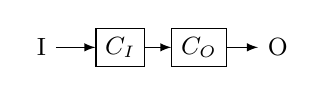
\begin{tikzpicture}[auto,>=latex]
  \node[] (I) {\code{I}};
  \node[block, right of=I] (CI) {$C_I$};
  \draw[->] (I) -- (CI);
  \node[block, right of=CI] (CO) {$C_O$};
  \node[right of=CO] (O) {\code{O}};
  \draw[->] (CI) -- (CO);
  \draw[->] (CO) -- (O);
\end{tikzpicture}
 &
 \parbox[b][][t]{\commentsize}{
  $C_I$ circuit for inner query, \\
   $C_O$ circuit for outer query.}
 \\[-3mm] \hline
Union &
\begin{lstlisting}[language=SQL]
(SELECT * FROM I1)
UNION
(SELECT * FROM I2)
\end{lstlisting}
&
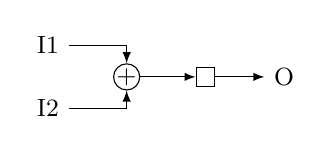
\begin{tikzpicture}[auto,>=latex]
  \node[] (input1) {\code{I1}};
  \node[below of=input1, node distance=.4cm] (midway) {};
  \node[below of=midway, node distance=.4cm] (input2) {\code{I2}};
  \node[block, shape=circle, right of=midway, inner sep=0in] (plus) {$+$};
  \node[block, right of=plus] (distinct) {$\distinct$};
  \node[right of=distinct] (output) {\code{O}};
  \draw[->] (input1) -| (plus);
  \draw[->] (input2) -| (plus);
  \draw[->] (plus) -- (distinct);
  \draw[->] (distinct) -- (output);
\end{tikzpicture}
& $\distinct$ eliminates duplicates.  An implementation of
\texttt{UNION ALL} does not need the $\distinct$.
\\[-3mm] \hline
Projection &
\begin{lstlisting}[language=SQL]
SELECT DISTINCT I.c
FROM I
\end{lstlisting}
&
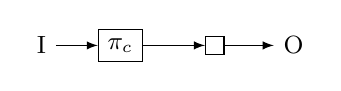
\begin{tikzpicture}[auto,>=latex]
  \node[] (input) {\code{I}};
  \node[block, right of=input] (pi) {$\pi_c$};
  \node[block, right of=pi, node distance=1.2cm] (distinct) {$\distinct$};
  \node[right of=distinct] (output) {\code{O}};
  \draw[->] (input) -- (pi);
  \draw[->] (pi) -- (distinct);
  \draw[->] (distinct) -- (output);
\end{tikzpicture}
&
\parbox[b][][t]{\commentsize}{
  Project each row with its weight unchanged.
  Add up weights of identical rows.
}
\\[-3mm] \hline
Filtering &
\begin{lstlisting}[language=SQL]
SELECT * FROM I
WHERE P(...)
\end{lstlisting}
&
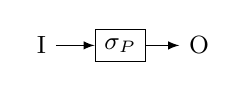
\begin{tikzpicture}[auto,>=latex]
  \node[] (input) {\code{I}};
  \node[block, right of=input] (map) {$\sigma_P$};
  \node[right of=map] (output) {\code{O}};
  \draw[->] (input) -- (map);
  \draw[->] (map) -- (output);
\end{tikzpicture}
&
\parbox[b][][t]{\commentsize}{
  P is a predicate applied to each row.
  Select each row separately.  If the row is selected, preserve the
  weight, else make the weight 0.
}
\\[-3mm] \hline
\parbox[b][][t]{1cm}{
Cartesian \\
product} &
\begin{lstlisting}[language=SQL]
SELECT I1.*, I2.*
FROM I1, I2
\end{lstlisting}
&
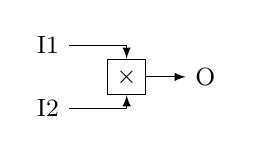
\begin{tikzpicture}[auto,>=latex]
  \node[] (i1) {\code{I1}};
  \node[below of=i1, node distance=.4cm] (midway) {};
  \node[below of=midway, node distance=.4cm] (i2) {\code{I2}};
  \node[block, right of=midway] (prod) {$\times$};
  \node[right of=prod] (output) {\code{O}};
  \draw[->] (i1) -| (prod);
  \draw[->] (i2) -| (prod);
  \draw[->] (prod) -- (output);
\end{tikzpicture}
&
\parbox[b][][t]{\commentsize}{
  The weight of the pair (a,b) is the product of the the weights of a
  and b.
}
\\[-1mm] \hline
Equi-join &
\begin{lstlisting}[language=SQL]
SELECT I1.*, I2.*
FROM I1 JOIN I2
ON I1.c1 = I2.c2
\end{lstlisting}
&
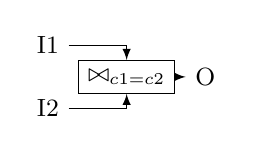
\begin{tikzpicture}[auto,>=latex]
  \node[] (i1) {\code{I1}};
  \node[below of=i1, node distance=.4cm] (midway) {};
  \node[below of=midway, node distance=.4cm] (i2) {\code{I2}};
  \node[block, right of=midway] (prod) {$\bowtie_{c1 = c2}$};
  \node[right of=prod] (output) {\code{O}};
  \draw[->] (i1) -| (prod);
  \draw[->] (i2) -| (prod);
  \draw[->] (prod) -- (output);
\end{tikzpicture}
&
\parbox[b][][t]{\commentsize}{
  Multiply the weights of the rows that appear in the output.
}
\\[-3mm] \hline
Intersection &
\begin{lstlisting}[language=SQL]
(SELECT * FROM I1)
INTERSECT
(SELECT * FROM I2)
\end{lstlisting}
&
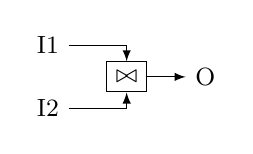
\begin{tikzpicture}[auto,>=latex]
  \node[] (i1) {\code{I1}};
  \node[below of=i1, node distance=.4cm] (midway) {};
  \node[below of=midway, node distance=.4cm] (i2) {\code{I2}};
  \node[block, right of=midway] (prod) {$\bowtie$};
  \node[right of=prod] (output) {\code{O}};
  \draw[->] (i1) -| (prod);
  \draw[->] (i2) -| (prod);
  \draw[->] (prod) -- (output);
\end{tikzpicture}
&
Special case of equi-join when both relations have the same schema.
 \\[-3mm] \hline
Difference &
\begin{lstlisting}[language=SQL]
SELECT * FROM I1
EXCEPT
SELECT * FROM I2
\end{lstlisting}
&
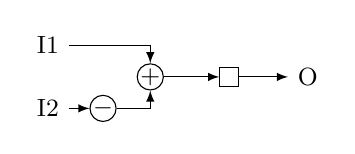
\begin{tikzpicture}[auto,>=latex, node distance=.7cm]
  \node[] (i1) {\code{I1}};
  \node[below of=i1, node distance=.4cm] (midway) {};
  \node[below of=midway, node distance=.4cm] (i2) {\code{I2}};
  \node[block, shape=circle, inner sep=0in, right of=i2] (m) {$-$};
  \node[block, right of=midway, shape=circle, inner sep=0in, node distance=1.3cm] (plus) {$+$};
  \node[block, right of=plus, node distance=1cm] (distinct) {$\distinct$};
  \node[right of=distinct, node distance=1cm] (output) {\code{O}};
  \draw[->] (i1) -| (plus);
  \draw[->] (i2) -- (m);
  \draw[->] (m) -| (plus);
  \draw[->] (plus) -- (distinct);
  \draw[->] (distinct) -- (output);
\end{tikzpicture}
&
$\distinct$ removes rows with negative weights from the result.
\\ \hline
\end{tabular}
\vspace{-3ex}
\end{table*}

In this section we apply the results on incremental computation to
relational databases.  As explained in the introduction, our goal is
to efficiently compute the incremental version of any relational query
$Q$.

However, we face a technical problem: we said that streams require
their values to belong to a commutative group, and relational
databases in general are \emph{not} commutative groups, since they
operate on sets.  Fortunately, there is a well-known tool in the
database literature which converts set operations into group
operations by using \zrs (also called z-relations~\cite{green-tcs11})
to represent sets.

\subsection{\zrs}

\zrs generalize database tables: think of a \zr as a table where each
row has an associated integer weight, possibly negative.  This weight
indicates \emph{how many times} the row belongs to the table.

%Given a set $A$, we define \defined{\zrs} over $A$ as functions with
%\emph{finite support} from $A$ to $\Z$.  These are functions $f: A
%\rightarrow \Z$ where $f(x) \not= 0$ for at most a finite number of
%values $x \in A$.  We also write $\Z[A]$ for the type of \zrs with
%elements from $A$.  Values in $\Z[A]$ can be thought of as key-value
%maps with keys in $A$ and values in $\Z$, justifying the array
%indexing notation.  If $m \in \Z[A]$ we write $m[a]$ instead of
%$m(a)$, again using an indexing notation.
%
%A particular \zr $m \in \Z[A]$ can be denoted by enumerating its
%elements that have non-zero weights and their corresponding weights:
%$m = \{ x_1 \mapsto w_1, \dots, x_n \mapsto w_n \}$.
%We call $w_i \in \Z$ the \defined{weight}
%of $x_i \in A$.  Weights can be negative.
%We write that $x \in m$ iff $m[x] \not= 0$.
%We also write $w \cdot x$ for $\{ x \mapsto w \}$.

%\ifzsetexamples
%Consider a concrete \zr $R \in \Z[\texttt{string}]$,
%defined by $R = \{ \texttt{joe} \mapsto 1, \texttt{anne} \mapsto -1 \}$.
%$R$ has two elements in its domain,
%\texttt{joe} with weight 1 (so $R[\texttt{joe}] = 1$),
%and \texttt{anne} with weight $-1$.
%We say \texttt{joe} $\in R$ and \texttt{anne} $\in R$.
%\fi

The following table shows an example \zr with three rows.  The first
row has value \texttt{joe} and weight 1.  We do not show rows with
weight 0.
%
\begin{center}
\begin{tabular}{|c|c|}\hline
  Row & Weight \\ \hline
  joe & 1 \\
  mary & 2 \\
  anne & -1 \\ \hline
\end{tabular}
\end{center}

%Since $\Z$ is an abelian ring, $\Z[A]$ is also an abelian ring (and thus a group).  This group
%$(\Z[A], +_{\Z[A]}, 0_{\Z[A]}, -_{\Z{A}})$ has addition and subtraction defined pointwise:
%$(f +_{\Z[A]} g)(x) = f(x) + g(x) . \forall x \in A.$
%The $0$ element of $\Z[A]$ is the function $0_{\Z[A]}$ defined by $0_{\Z[A]}(x) = 0 .
%\forall x \in A$.  For example, $R + R =  \{ \texttt{joe} \mapsto 2, \texttt{anne} \mapsto -2 \}$.
%Since \zrs form a group, all results from \secref{sec:streams} apply to streams over \zrs.

\zrs generalize sets and multisets: a set can be represented as a \zr
by associating a weight of 1 with each element.  Multisets (also
called ``bags'' in the database literature) are \zrs where all weights
are positive.  Crucially, \zrs can also represent \emph{changes} to
sets and bags.  Negative weights represent rows that are being
\emph{removed}.

We can define three operations on \zrs with values of a given type:
(1) \textbf{zero} (a \zr with all weights 0) (2) \textbf{negation}:
just negate all weights; (3) \textbf{plus}: add up the weights of the
rows that have the same value.  Using these operations \zrs are a
commutative group.

%\begin{definition}
%We say that a \zr represents a \defined{set} if the weight of every
%element is one.  We define a function to check this property
%$\isset : \Z[A] \rightarrow \B$\index{isset}
%given by:
%$$\isset(m) \defn \left\{
%\begin{array}{ll}
%  \mbox{true} & \mbox{ if } m[x] = 1, \forall x \in m \\
%  \mbox{false} & \mbox{ otherwise}
%\end{array}
%\right.
%$$
%\end{definition}

%\ifzsetexamples
%For our example $\isset(R) = \mbox{false}$, since $R[\texttt{anne}] = -1$.
%\fi

%\begin{definition}
%We say that a \zr is \defined{positive} (or a \defined{bag}) if the weight of every element is
%positive.  We define a function to check this property
%$\ispositive : \Z[A] \rightarrow \B$\index{ispositive}.
%given by
%$$\ispositive(m) \defn \left\{
%\begin{array}{ll}
%  \mbox{true} & \mbox{ if } m[x] \geq 0, \forall x \in A \\
%  \mbox{false} & \mbox{ otherwise}
%\end{array}
%\right.$$
%\end{definition}
%We have $\forall m \in \Z[A] . \isset(m) \Rightarrow \ispositive(m)$.
%\ifzsetexamples
%$\ispositive(R) = \mbox{false}$, since $R[\texttt{anne}] = -1$.
%\fi
%
%We write $m \geq 0$ when $m$ is positive.  For positive $m, n \in
%\Z[A]$ we write $m \geq n$ for iff $m - n \geq 0$.  $\geq$ is a
%partial order.
%
%We call a function $f : \Z[A] \rightarrow \Z[B]$ \defined{positive} if it maps
%positive values to positive values:
%$\forall x \in \Z[A], x \geq 0_{\Z[A]} \Rightarrow f(x) \geq 0_{\Z[B]}$.
%We use the same notation for functions: $\ispositive(f)$.

%\begin{definition}[distinct]
%The function $\distinct: \Z[A] \rightarrow \Z[A]$\index{distinct}
%``converts'' a \zr into a set:
%$$\distinct(m)[x] \defn \left\{
%\begin{array}{ll}
%  1 & \mbox{ if } m[x] > 0 \\
%  0 & \mbox{ otherwise}
%\end{array}
%\right.
%$$
%%\end{definition}

We define the function $\distinct$ on \zrs. This function's output is
a \zr where all rows of the input with negative weights are removed,
and all positive weights are changed to 1.  For example, the
$\distinct$ of the above \zr is:
%
\begin{center}
\begin{tabular}{|c|c|}\hline
  Row & Weight \\ \hline
  joe & 1 \\
  mary & 1 \\ \hline
\end{tabular}
\end{center}

Notice that $\distinct$ ``removes'' duplicates from multisets, and it also eliminates
rows with negative weights.
%\ifzsetexamples
%$\distinct(R) = \{ \texttt{joe} \mapsto 1 \}$.
%\fi

\subsection{Implementing relational operators}\label{sec:relational-operators}

The fact that relational algebra can be implemented by computations on
\zrs has been shown before, e.g.~\cite{green-pods07}.  The translation
of the relational operators to functions computing on \zrs is shown in
Table~\ref{tab:relational}.  The functions ($\pi$, $\sigma$,
$\bowtie$, $\times$) are the standard relational operators projection,
selection, join, Cartesian product.  The first row of the table shows
that a composite query is translated recursively: implement the
sub-queries, and connect them with an arrow.  This gives us a recipe
for translating an arbitrary relational query plan into a circuit.

The translation is fairly straightforward, but many operators require
the application of a $\distinct$ \textbf{to produce sets}.  For
example, $a \cup b = \distinct(a + b)$, $a \setminus b = \distinct(a -
b)$.  Filtering on \zrs works exactly as filtering on sets, but
preserves the weight of each value.  Selection on \zrs works similar
to selection on sets, but also preserves the weights.

%\paragraph{Correctness of the \dbsp implementations}\label{sec:correctness}
%
%A relational query $Q$ that transforms
%a set $V$ into a set $U$ is implemented by a \dbsp computation $Q'$ on
%\zrs.  The correctness of the implementation requires the following
%diagram to commute:
%
%\begin{center}
%\begin{tikzpicture}
%  \node[] (V) {$V$};
%  \node[below of=V] (VZ) {$VZ$};
%  \node[right of=V, node distance=2cm] (U) {$U$};
%  \node[below of=U] (UZ) {$UZ$};
%  \draw[->] (V) -- node (f) [below] {$Q$} (U);
%  \draw[->] (V) --  node (s) [left] {tozset}(VZ);
%  \draw[->] (VZ) -- node (f) [above] {$Q'$} (UZ);
%  \draw[->] (UZ) -- node (d) [right] {toset} (U);
%\end{tikzpicture}
%\end{center}
%
%(The correctness of
%this implementation is predicated on $Q'$'s inputs being
%sets, an invariant which needs to be maintained by the environment.)
%The ``$\mbox{toset}$'' and ``$\mbox{tozset}$'' functions convert sets to \zrs and
%vice-versa, in the expected way:
%
%$\mbox{toset}: \Z[A] \to 2^A$ is defined as $\mbox{toset}(m) \defn \cup_{x \in \distinct(m)} \{ x \}$.
%
%$\mbox{tozset}: 2^A \to \Z[A]$ is defined as $\mbox{tozset}(s) \defn \sum_{x \in s} 1 \cdot x$.
%
%All standard algebraic properties
%of the relational operators can be used to optimize circuits
%(they can even be applied to queries before building the circuits).

This is a faithful implementation of the relational algebra --- the
underlying mathematical theory that underlies modern databases ---
using \zrs.  This implementation produces an abundance of $\distinct$
operators, but there are known optimizations for removing some of
them.

The following functions in Table~\ref{tab:relational} are linear:
$\sigma, \pi, -, +$.  The following functions are bilinear: $\times,
\bowtie$.  In fact, the only non-linear function is $\distinct$.  In
consequence, all these functions (lifted) have very efficient
incremental versions.

To explain why these functions are linear, consider the filtering
query from the introduction (\texttt{WHERE}).  What is the change in
the output when we add a new row to the input?  It is sufficient to
check the predicate for the new row.  If the predicate returns
\texttt{true}, the new row is added to the output.  So the change in
the output only depends on the change in the input, and not on the
actual contents of the input.  This is what makes the operation
linear.

%Prior work (e.g., Proposition 6.13 in~\cite{green-tcs11}) has shown
%how some invocations of $\distinct$ can be eliminated from query plans
%without changing the query semantics; we will see that incremental
%versions of $\distinct$ operators incur significant space costs.
%
%\begin{proposition}\label{prop-distinct-delay}
%Let $Q$ be one of the following \zrs operators: filtering $\sigma$,
%join $\bowtie$, or Cartesian product $\times$.
%Then we have $\forall i \in \Z[I], \ispositive(i) \Rightarrow Q(\distinct(i)) = \distinct(Q(i))$.
%\end{proposition}
%
%\begin{comment}
%\noindent
%\begin{tabular}{m{3.5cm}m{.5cm}m{3.5cm}}
%\begin{tikzpicture}[auto,>=latex]
%  \node[] (input) {$i$};
%  \node[block, right of=input, node distance=1.1cm] (distinct) {$\distinct$};
%  \node[block, right of=distinct, node distance=1.2cm] (q) {$Q$};
%  \node[right of=q] (output)  {$o$};
%  \draw[->] (input) -- (distinct);
%  \draw[->] (distinct) -- (q);
%  \draw[->] (q) -- (output);
%\end{tikzpicture}
%&
%$\cong$
%&
%\begin{tikzpicture}[auto,>=latex]
%  \node[] (input) {$i$};
%  \node[block, right of=input] (q) {$Q$};
%  \node[block, right of=q, node distance=1.2cm] (distinct1) {$\distinct$};
%  \node[right of=distinct1, node distance=1.2cm] (output)  {$o$};
%  \draw[->] (input) -- (q);
%  \draw[->] (q) -- (distinct1);
%  \draw[->] (distinct1) -- (output);
%\end{tikzpicture}
%\end{tabular}
%
%This rule allows us to delay the application of $\distinct$.
%\end{comment}
%
%\begin{proposition}\label{prop-distinct-once}
%Let $Q$ be one of the following \zrs operators: filtering $\sigma$,
%projection $\pi$, map($f$)\footnote{Technically, map (applying a user-defined
%function to each row) is not relational.},
%addition $+$, join $\bowtie$, or
%Cartesian product $\times$.
%Then we have $\ispositive(i) \Rightarrow \distinct(Q(\distinct(i))) = \distinct(Q(i))$.
%\end{proposition}
%
%\begin{comment}
%\noindent
%\begin{tabular}{m{6.5cm}m{.5cm}}
%\begin{tikzpicture}[auto,>=latex]
%  \node[] (input) {$i$};
%  \node[block, right of=input, node distance=1.5cm] (distinct) {$\distinct$};
%  \node[block, right of=distinct, node distance=1.5cm] (q) {$Q$};
%  \node[block, right of=q, node distance=1.5cm] (distinct1) {$\distinct$};
%  \node[right of=distinct1, node distance=1.5cm] (output)  {$o$};
%  \draw[->] (input) -- (distinct);
%  \draw[->] (distinct) -- (q);
%  \draw[->] (q) -- (distinct1);
%  \draw[->] (distinct1) -- (output);
%\end{tikzpicture}
%&
%$\cong$ \\
%\begin{tikzpicture}[auto,>=latex]
%  \node[] (input) {$i$};
%  \node[block, right of=input] (q) {$Q$};
%  \node[block, right of=q, node distance=1.5cm] (distinct1) {$\distinct$};
%  \node[right of=distinct1, node distance=1.5cm] (output)  {$o$};
%  \draw[->] (input) -- (q);
%  \draw[->] (q) -- (distinct1);
%  \draw[->] (distinct1) -- (output);
%\end{tikzpicture}
%\end{tabular}
%\end{comment}
%
%These properties allow us to ``consolidate'' distinct operators by performing
%one $\distinct$ at the end of a chain of computations.

\subsection{Incremental view maintenance}

Let us consider a relational query $Q$ defining a view $V$.  To the
following algorithm builds a \dbsp circuit for $\inc{Q}$:
%
\begin{algorithm}[incremental view maintenance]\label{algorithm-inc}\!
  \vspace{-3mm}
\begin{enumerate}[nosep, leftmargin=0pt, itemindent=0.5cm, label=\textbf{(\arabic{*})}]
\item Translate $Q$ into a circuit using the rules in Table~\ref{tab:relational}.
\item{} [Optional] Remove some $\distinct$ operations.
\item Lift the whole circuit, converting it to a circuit operating
  on streams, using formula (**) in \refsec{sec:streams}.
\item Incrementalize the circuit ``surrounding'' it with $\I$ and $\D$.
\item Apply the chain rule recursively, producing a circuit using only
  primitive incremental operations.
\end{enumerate}
\end{algorithm}

This algorithm is deterministic; the running time is proportional to
the number of operators in the query.  Step (2) generates an
equivalent circuit, with fewer $\distinct$ operators.  Step (3) yields
a circuit that consumes a \emph{stream} of complete database snapshots
and outputs a stream of view snapshots. Step (4) yields a circuit that
consumes a stream of \emph{database changes} and outputs a stream of
\emph{view changes}; however, the internal operation of the circuit is
non-incremental, as it rebuilds the complete database using
integrations.  Step (5) optimizes the circuit by replacing each
primitive operator with its incremental version.  It essentially adds
a $\I \circ \D$ pair on every edge in the circuit, and then uses the
chain rule to replace each $\I \circ Q \circ \D$ with $\inc{Q}$.

After running this algorithm, all primitives operations are replaced
by their incremental versions.  The only non-linear operation from
Table~\ref{tab:relational} is $\distinct$.  However, there is an
efficient incremental implementation for $\distinct$ (this
construction has also been known before, but we show it in terms of
streaming operations), shown in the following diagram:

\noindent
\begin{tabular}{m{3.9cm}m{0cm}m{5cm}}
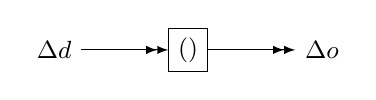
\begin{tikzpicture}[auto,node distance=1.7cm,>=latex]
    \node[] (input) {$\Delta d$};
    \node[block, right of=input] (d) {$\inc{(\lift{\distinct})}$};
    \node[right of=d] (output) {$\Delta o$};
    \draw[->>] (input) -- (d);
    \draw[->>] (d) -- (output);
\end{tikzpicture} &
$\cong$ &
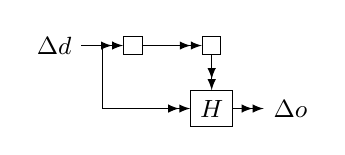
\begin{tikzpicture}[>=latex]
    \node[] (input) {$\Delta d$};
    \node[block, right of=input] (I) {$\I$};
    \node[block, right of=I] (z) {$\zm$};
    \node[block, below of=z, node distance=.8cm] (H) {$\lift{H}$};
    \node[right of=H] (output) {$\Delta o$};
    \draw[->>] (input) -- node (mid) {} (I);
    \draw[->>] (I) -- (z);
    \draw[->>] (mid.center) |- (H);
    \draw[->>] (z) -- node (i) [right] {} (H);
    \draw[->>] (H) -- (output);
\end{tikzpicture}
\end{tabular}

%\noindent where $H: \Z[A] \times \Z[A] \to \Z[A]$ is defined as: \\
%$$
%H(i, d)[x] \defn
%\begin{cases}
%-1 & \mbox{if } i[x] > 0 \mbox{ and } (i + d)[x] \leq 0 \\
%1  & \mbox{if } i[x] \leq 0 \mbox{ and } (i + d)[x] > 0 \\
%0  & \mbox{otherwise} \\
%\end{cases}
%$$
%\end{proposition}

The function $H$ has two inputs: the left input is the change $\Delta
d$, while the top input is the full set, obtained as an integral of
the changes.  $H$ detects whether the weight of a row in the full set
is changing sign (from negative to positive on a row insertion, and
from positive to negative on a deletion) when the row appears in a new
change.  Here is the intuition why $\distinct$ is efficiently
incrementalizable: only tuples that appear in the input change $\Delta
d$ can appear in the output change $\Delta o$, so the work performed
is $O(|\Delta d)|$.  The implementation needs to maintain the
\emph{entire input set} (similar to joins) in order to discover
whether an item is new or not.  That is the purpose of the $\I$
operator.

The algorithm reduces the problem of incremental execution of a query
plan to the incremental execution of sub\-plans/primitive operators.
However, this algorithm works even if we use a primitive $P$ for which
no efficient incremental version is known: we can always use the
inefficient ``brute-force'' implementation given by $\inc{P} = \D
\circ \lift{P} \circ \I$.

\subsection{Relational Query Example}\label{sec:relational-example}

Let's apply the IVM algorithm to the following SQL query:
\begin{lstlisting}[language=SQL,basicstyle=\small\ttfamily]
CREATE VIEW v AS
SELECT DISTINCT a.x, b.y FROM (
     SELECT t1.x, t1.id FROM t1 WHERE t1.a > 2
) a JOIN (
     SELECT t2.id, t2.y FROM t2 WHERE t2.s > 5
) b ON a.id = b.id
\end{lstlisting}

\vspace{-1.6ex}

Step 1: Create a \dbsp circuit to represent this query using the rules
in Table~\ref{tab:relational}; this circuit is essentially a dataflow
implementation of the query:

\noindent
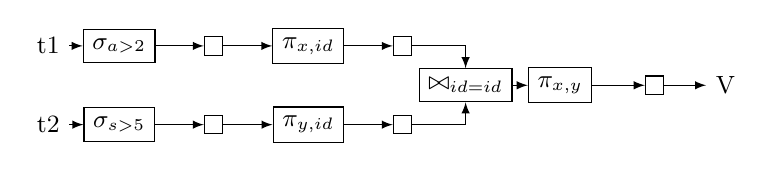
\begin{tikzpicture}[node distance=1.2cm,>=latex]
    \node[] (t1) {\code{t1}};
    \node[block, right of=t1, node distance=.9cm] (s1) {$\sigma_{a > 2}$};
    \node[block, right of=s1] (d1) {$\distinct$};
    \node[block, right of=d1] (p1) {$\pi_{x, id}$};
    \node[block, right of=p1] (d11) {$\distinct$};
    \node[below of=t1, node distance=1cm] (t2) {\code{t2}};
    \node[block, right of=t2, node distance=.9cm] (s2) {$\sigma_{s > 5}$};
    \node[block, right of=s2] (d2) {$\distinct$};
    \node[block, right of=d2] (p2) {$\pi_{y, id}$};
    \node[block, right of=p2] (d21) {$\distinct$};
    \node[below of=d11, node distance=.5cm] (mid) {};
    \node[block, right of=mid, node distance=.8cm] (j) {$\bowtie_{id = id}$};
    \node[block, right of=j] (p) {$\pi_{x, y}$};
    \node[block, right of=p] (d) {$\distinct$};
    \node[right of=d, node distance=.9cm] (V) {\code{V}};
    \draw[->] (t1) -- (s1);
    \draw[->] (s1) -- (d1);
    \draw[->] (d1) -- (p1);
    \draw[->] (p1) -- (d11);
    \draw[->] (t2) -- (s2);
    \draw[->] (s2) -- (d2);
    \draw[->] (d2) -- (p2);
    \draw[->] (p2) -- (d21);
    \draw[->] (d11) -| (j);
    \draw[->] (d21) -| (j);
    \draw[->] (j) -- (p);
    \draw[->] (p) -- (d);
    \draw[->] (d) -- (V);
\end{tikzpicture}

Step 2: eliminate $\distinct$ operators, producing an equivalent
circuit: (we omit the subscripts to save space):

%\noindent
%\begin{tikzpicture}[node distance=1.2cm,>=latex]
%    \node[] (t1) {\code{t1}};
%    \node[block, right of=t1, node distance=.9cm] (s1) {$\sigma_{a > 2}$};
%    \node[block, right of=s1] (p1) {$\pi_{x, id}$};
%    \node[block, right of=p1] (d11) {$\distinct$};
%    \node[below of=t1, node distance=1cm] (t2) {\code{t2}};
%    \node[block, right of=t2, node distance=.9cm] (s2) {$\sigma_{s > 5}$};
%    \node[block, right of=s2] (p2) {$\pi_{y, id}$};
%    \node[block, right of=p2] (d21) {$\distinct$};
%    \node[below of=d11, node distance=.5cm] (mid) {};
%    \node[block, right of=mid, node distance=.8cm] (j) {$\bowtie_{id = id}$};
%    \node[block, right of=j] (p) {$\pi_{x, y}$};
%    \node[block, right of=p] (d) {$\distinct$};
%    \node[right of=d, node distance=1.2cm] (V) {\code{V}};
%    \draw[->] (t1) -- (s1);
%    \draw[->] (s1) -- (p1);
%    \draw[->] (p1) -- (d11);
%    \draw[->] (t2) -- (s2);
%    \draw[->] (s2) -- (p2);
%    \draw[->] (p2) -- (d21);
%    \draw[->] (d11) -| (j);
%    \draw[->] (d21) -| (j);
%    \draw[->] (j) -- (p);
%    \draw[->] (p) -- (d);
%    \draw[->] (d) -- (V);
%\end{tikzpicture}


%\noindent
%\begin{tikzpicture}[node distance=1.2cm,>=latex]
%    \node[] (t1) {\code{t1}};
%    \node[block, right of=t1, node distance=.9cm] (s1) {$\sigma$};
%    \node[block, right of=s1] (p1) {$\pi$};
%    \node[below of=t1, node distance=1cm] (t2) {\code{t2}};
%    \node[block, right of=t2, node distance=.9cm] (s2) {$\sigma$};
%    \node[block, right of=s2] (p2) {$\pi$};
%    \node[below of=p1, node distance=.5cm] (mid) {};
%    \node[block, right of=mid, node distance=.8cm] (j) {$\bowtie$};
%    \node[block, right of=j] (d0) {$\distinct$};
%    \node[block, right of=d0] (p) {$\pi$};
%    \node[block, right of=p] (d) {$\distinct$};
%    \node[right of=d, node distance=1.2cm] (V) {\code{V}};
%    \draw[->] (t1) -- (s1);
%    \draw[->] (s1) -- (p1);
%    \draw[->] (t2) -- (s2);
%    \draw[->] (s2) -- (p2);
%    \draw[->] (p1) -| (j);
%    \draw[->] (p2) -| (j);
%    \draw[->] (j) -- (d0);
%    \draw[->] (d0) -- (p);
%    \draw[->] (p) -- (d);
%    \draw[->] (d) -- (V);
%\end{tikzpicture}
%
%\noindent And again~\ref{prop-distinct-once}:

\noindent
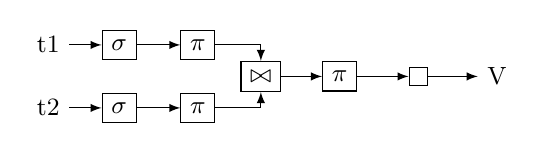
\begin{tikzpicture}[node distance=1cm,>=latex]
  \node[] (t1) {\code{t1}};
  \node[block, right of=t1, node distance=.9cm] (s1) {$\sigma$};
  \node[block, right of=s1] (p1) {$\pi$};
  \node[below of=t1, node distance=.8cm] (t2) {\code{t2}};
  \node[block, right of=t2, node distance=.9cm] (s2) {$\sigma$};
  \node[block, right of=s2] (p2) {$\pi$};
  \node[below of=p1, node distance=.4cm] (mid) {};
  \node[block, right of=mid, node distance=.8cm] (j) {$\bowtie$};
  \node[block, right of=j] (p) {$\pi$};
  \node[block, right of=p] (d) {$\distinct$};
  \node[right of=d, node distance=1cm] (V) {\code{V}};
  \draw[->] (t1) -- (s1);
  \draw[->] (s1) -- (p1);
  \draw[->] (t2) -- (s2);
  \draw[->] (s2) -- (p2);
  \draw[->] (p1) -| (j);
  \draw[->] (p2) -| (j);
  \draw[->] (j) -- (p);
  \draw[->] (p) -- (d);
  \draw[->] (d) -- (V);
\end{tikzpicture}

This step is used in some traditional database optimizers.  Note that
some arrows that represented sets in the original circuit may
represent multisets in the optimized circuit.

Step 3: lift the circuit to compute over streams; all arrows are
doubled and all functions are lifted:

\noindent
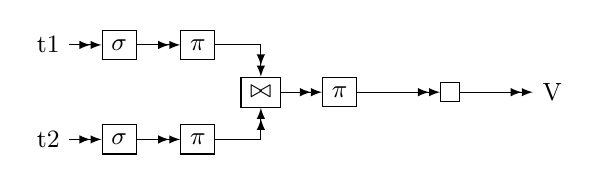
\begin{tikzpicture}[node distance=1cm,>=latex]
    \node[] (t1) {\code{t1}};
    \node[block, right of=t1, node distance=.9cm] (s1) {$\lift{\sigma}$};
    \node[block, right of=s1] (p1) {$\lift{\pi}$};
    \node[below of=t1, node distance=1.2cm] (t2) {\code{t2}};
    \node[block, right of=t2, node distance=.9cm] (s2) {$\lift{\sigma}$};
    \node[block, right of=s2] (p2) {$\lift{\pi}$};
    \node[below of=p1, node distance=.6cm] (mid) {};
    \node[block, right of=mid, node distance=.8cm] (j) {$\lift{\bowtie}$};
    \node[block, right of=j] (p) {$\lift{\pi}$};
    \node[block, right of=p, node distance=1.4cm] (d) {$\lift{\distinct}$};
    \node[right of=d, node distance=1.3cm] (V) {\code{V}};
    \draw[->>] (t1) -- (s1);
    \draw[->>] (s1) -- (p1);
    \draw[->>] (t2) -- (s2);
    \draw[->>] (s2) -- (p2);
    \draw[->>] (p1) -| (j);
    \draw[->>] (p2) -| (j);
    \draw[->>] (j) -- (p);
    \draw[->>] (p) -- (d);
    \draw[->>] (d) -- (V);
\end{tikzpicture}

Step 4: incrementalize circuit, obtaining a circuit that computes over changes;
this circuit receives changes to relations \code{t1} and \code{t2} and for each
such change it produces the corresponding change in the output view \code{V}:

\noindent
\begin{tikzpicture}[node distance=1cm,>=latex]
    \node[] (t1) {$\Delta$\code{t1}};
    \node[block, right of=t1, node distance=.8cm] (I1) {$\I$};
    \node[block, right of=I1, node distance=.9cm] (s1) {$\lift{\sigma}$};
    \node[block, right of=s1] (p1) {$\lift{\pi}$};
    \node[below of=t1, node distance=1.2cm] (t2) {$\Delta$\code{t2}};
    \node[block, right of=t2, node distance=.8cm] (I2) {$\I$};
    \node[block, right of=I2, node distance=.9cm] (s2) {$\lift{\sigma}$};
    \node[block, right of=s2] (p2) {$\lift{\pi}$};
    \node[below of=p1, node distance=.6cm] (mid) {};
    \node[block, right of=mid, node distance=.7cm] (j) {$\lift{\bowtie}$};
    \node[block, right of=j] (p) {$\lift{\pi}$};
    \node[block, right of=p, node distance=1.4cm] (d) {$\lift{\distinct}$};
    \node[block, right of=d, node distance=1.3cm] (D) {$\D$};
    \node[right of=D, node distance=.8cm] (V) {$\Delta$\code{V}};
    \draw[->>] (t1) -- (I1);
    \draw[->>] (I1) -- (s1);
    \draw[->>] (s1) -- (p1);
    \draw[->>] (t2) -- (I2);
    \draw[->>] (I2) -- (s2);
    \draw[->>] (s2) -- (p2);
    \draw[->>] (p1) -| (j);
    \draw[->>] (p2) -| (j);
    \draw[->>] (j) -- (p);
    \draw[->>] (p) -- (d);
    \draw[->>] (d) -- (D);
    \draw[->>] (D) -- (V);
\end{tikzpicture}

Step 5: apply the chain rule to rewrite the circuit as a composition
of incremental operators; notice the use of $\inc{.}$ for all
operators:

\noindent
\begin{tikzpicture}[node distance=1.6cm,>=latex]
    \node[] (t1) {$\Delta$\code{t1}};
    \node[block, right of=t1, node distance=1.2cm] (s1) {$\inc{(\lift{\sigma})}$};
    \node[block, right of=s1, node distance=1.4cm] (p1) {$\inc{(\lift{\pi})}$};
    \node[below of=t1, node distance=1.2cm] (t2) {$\Delta$\code{t2}};
    \node[block, right of=t2, node distance=1.2cm] (s2) {$\inc{(\lift{\sigma})}$};
    \node[block, right of=s2, node distance=1.4cm] (p2) {$\inc{(\lift{\pi})}$};
    \node[below of=p1, node distance=.6cm] (mid) {};
    \node[block, right of=mid, node distance=.6cm] (j) {$\inc{(\lift{\bowtie})}$};
    \node[block, right of=j,node distance=1.4cm] (p) {$\inc{(\lift{\pi})}$};
    \node[block, right of=p,node distance=1.7cm] (d) {$\inc{(\lift{\distinct})}$};
    \node[right of=d, node distance=1.5cm] (V) {$\Delta$\code{V}};
    \draw[->>] (t1) -- (s1);
    \draw[->>] (s1) -- (p1);
    \draw[->>] (t2) -- (s2);
    \draw[->>] (s2) -- (p2);
    \draw[->>] (p1) -| (j);
    \draw[->>] (p2) -| (j);
    \draw[->>] (j) -- (p);
    \draw[->>] (p) -- (d);
    \draw[->>] (d) -- (V);
\end{tikzpicture}

Use the linearity of $\sigma$ and $\pi$ to simplify this circuit (notice that
all linear operators no longer have a $\inc{\cdot}$):

\noindent
\begin{tikzpicture}[node distance=1cm,>=latex]
    \node[] (t1) {$\Delta$\code{t1}};
    \node[block, right of=t1, node distance=1cm] (s1) {$\lift{\sigma}$};
    \node[block, right of=s1] (p1) {$\lift{\pi}$};
    \node[below of=t1, node distance=1.2cm] (t2) {$\Delta$\code{t2}};
    \node[block, right of=t2, node distance=1cm] (s2) {$\lift{\sigma}$};
    \node[block, right of=s2] (p2) {$\lift{\pi}$};
    \node[below of=p1, node distance=.6cm] (mid) {};
    \node[block, right of=mid, node distance=.8cm] (j) {$\inc{(\lift{\bowtie})}$};
    \node[block, right of=j, node distance=1.2cm] (p) {$\lift{\pi}$};
    \node[block, right of=p, node distance=1.6cm] (d) {$\inc{(\lift{\distinct})}$};
    \node[right of=d, node distance=1.6cm] (V) {$\Delta$\code{V}};
    \draw[->>] (t1) -- (s1);
    \draw[->>] (s1) -- (p1);
    \draw[->>] (t2) -- (s2);
    \draw[->>] (s2) -- (p2);
    \draw[->>] (p1) -| (j);
    \draw[->>] (p2) -| (j);
    \draw[->>] (j) -- (p);
    \draw[->>] (p) -- (d);
    \draw[->>] (d) -- (V);
\end{tikzpicture}

Finally, replace the incremental join and the incremental $\distinct$,
with their incremental implementations, obtaining the following
circuit (we have used a slightly different expansion for the join than
the one shown previously; this one only contains two integrators):

\noindent
\begin{tikzpicture}[node distance=.8cm,>=latex]
    \node[] (t1) {$\Delta$\code{t1}};
    \node[block, right of=t1] (s1) {$\lift{\sigma}$};
    \node[block, right of=s1] (p1) {$\lift{\pi}$};
    \node[below of=t1, node distance=.8cm] (t2) {$\Delta$\code{t2}};
    \node[block, right of=t2] (s2) {$\lift{\sigma}$};
    \node[block, right of=s2] (p2) {$\lift{\pi}$};

    % join expansion
      \node[block, right of=p1] (jI1) {$\I$};
      \node[block, right of=p2] (jI2) {$\I$};
      \draw[->>] (p1) -- (jI1);
      \draw[->>] (p2) -- (jI2);
      \node[block, right of=jI2] (ZI2) {$\zm$};
      \draw[->>] (jI2) -- (ZI2);
      \node[block, right of=jI1] (DI1) {$\lift\bowtie$};
      \node[block, right of=ZI2, node distance=1cm] (DI2) {$\lift\bowtie$};
      \draw[->>] (jI1) -- (DI1);
      \draw[->>] (ZI2) -- (DI2);
      \node[block, circle, above of=DI2, inner sep=0cm] (sum) {$+$};
      \draw[->>] (DI1) -- (sum);
      \draw[->>] (DI2) -- (sum);
      \draw[->>] (p1) -- (DI2);
      \draw[->>] (p2) -- (DI1);

    \node[block, right of=sum] (p) {$\lift{\pi}$};
    \draw[->>] (sum) -- (p);
    \node[block, right of=p] (Id) {$\I$};
    \node[block, right of=Id, node distance=1cm] (zd) {$\zm$};
    \node[block, below of=zd] (H) {$\lift{H}$};
    \node[right of=H, node distance=1cm] (V) {$\Delta$\code{V}};
    \draw[->>] (t1) -- (s1);
    \draw[->>] (s1) -- (p1);
    \draw[->>] (t2) -- (s2);
    \draw[->>] (s2) -- (p2);
    \draw[->>] (p) -- node (tapp) {} (Id);
    \draw[->>] (Id) -- (zd);
    \draw[->>] (zd) -- (H);
    \draw[->>] (tapp.center) |- (H);
    \draw[->>] (H) -- (V);
\end{tikzpicture}

Notice that the resulting circuit contains three integration
operations: two from the join, and one from the $\distinct$.  It also
contains two join operators.  However, the work performed by each
operator for each new input is proportional to the size of its input
change.


%\refsec{sec:relational-example} shows a concrete example of a relational query converted
%into a circuit and then incrementalized using Algorithm~\ref{algorithm-inc}.

%\subsection{Complexity of incremental circuits}\label{sec:complexity}
%
%Incremental circuits are efficient.  We evaluate the cost of a circuit
%while processing the $t$-th input change.  Even if $Q$ is a pure
%function, $\inc{Q}$ is actually a streaming system, with internal
%state.  This state is stored entirely in the delay operators $\zm$,
%some of which appear in $\I$ and $\D$ operators.  The result produced
%by $\inc{Q}$ on the $t$-th input depends in general not only on the
%new $t$-th input, but also on all prior inputs it has received.
%
%We argue that each operator in the incremental version of a circuit is
%efficient in terms of work and space.  We make the standard IVM
%assumption that the input changes \emph{of each operator} are small:
%$|\Delta DB[t]| \ll |DB[t]| = |(\I(\Delta DB))[t]|$.
%
%An unoptimized incremental operator $\inc{Q} = \D \circ Q \circ \I$
%evaluates query $Q$ on the whole database $DB$, the integral of the input stream:
%$DB = \I(\Delta DB)$; hence its time complexity  is the same as that of the non-incremental
%evaluation of $Q$.  In addition, each of the $\I$ and $\D$ operators uses $O(|DB[t]|)$ memory.
%
%Step (5) of the incrementalization algorithm applies the optimizations described in \secref{sec:incremental};
%these reduce the time complexity of each operator to be a function of $O(|\Delta DB[t]|)$.
%For example, Theorem~\ref{linear}, allows evaluating $\inc{S}$, where $S$ is a
%linear operator, in time $O(|\Delta DB[t]|)$.  The $\I$
%operator can also be evaluated in $O(|\Delta DB[t]|)$ time, because
%all values that appear in the output of $\I(\Delta DB)[t]$ must be present in
%current input change $\Delta DB[t]$.  Similarly, while the $\distinct$ operator is not
%linear, $\inc{(\lift{\distinct})}$ can also be evaluated in $O(|\Delta DB[t]|)$ according to
%Proposition~\ref{prop-inc_distinct}.  Bilinear operators, including join, can be
%evaluated in time $O(|DB[t]| \times |\Delta DB[t]|)$, which is a factor of $|DB[t] / \Delta DB[t]|$
%better than full re-evaluation.
%
%The space complexity of linear operators is 0 (zero), since they store no
%data persistently.  The space complexity of operators such as $\inc{(\lift{\distinct})}$,
%$\inc{(\lift{\bowtie})}$, $\I$, and $\D$ is $O(|DB[t]|)$.  They need
%to store their input or output relations in full.

\subsection{SQL}

SQL is richer than the relational algebra.  It can perform operations
on multisets, and it offers operations such as \texttt{GROUP BY} and
aggregations.  All of these can be modeled as operations on \zr-like
structures.  Moreover, \texttt{GROUP BY} is a linear operation.  Some
aggregations are ``almost'' linear, but other, such as \texttt{MIN},
require maintaining the full input set, similar to $\distinct$, to
properly handle deletions.  See the full paper and the technical
report~\cite{tr} for more details.


\section{Recursive queries}\label{sec:recursion}

Recursive queries are very useful in many applications.  For
example, graph algorithms such as graph reachability or transitive
closure are naturally expressed using recursive queries.  We introduce
two simple \dbsp stream operators that are used for expressing
recursive query evaluation.  These operators allow us to build
circuits implementing looping constructs, which are used to iterate
computations until a fixed-point is reached (i.e., the output of some
operator does not change anymore).

\subsection{Creating and destroying streams}

%\begin{definition}\label{def:zae}
%We say that a stream $s \in \stream{A}$ is \defined{zero almost-everywhere} if it has a finite
%number of non-zero values, i.e., there exists a time $t_0 \in \N$
%s.t. $\forall t \geq t_0 . s[t] = 0$.
%\noindent Denote the set of streams that are zero almost everywhere
%by $\streamf{A} \subset \stream{A}$.
%\end{definition}

% \paragraph{Stream introduction}

The \defined{delta function} $\delta : A \rightarrow \stream{A}$
produces a stream from a scalar value.  Given an input value $x$, the
output stream is $x$ followed by an infinite number of zeros.  The
input of $\delta$ has a single arrow, while the output has a double
arrow.
%
%$$\delta(v)[t] \defn \left\{
%\begin{array}{ll}
%  v & \mbox{if } t = 0 \\
%  0_A & \mbox{ otherwise}
%\end{array}
%\right.
%$$
%\ifstreamexamples
%For example, $\delta(5)$ is the stream $\sv{5 0 0 0 0}$.
%\fi
\begin{center}
\begin{tikzpicture}[auto,node distance=1cm,>=latex]
    \node[] (input) {\fbox{x}};
    \node[block, right of=input] (delta) {$\delta$};
    \node[right of=delta, node distance=2.2cm] (output) {\sv{x 0 0 0 0}};
    \draw[->] (input) -- (delta);
    \draw[->>] (delta) -- (output);
\end{tikzpicture}
\end{center}

% \paragraph{Stream elimination}

We define the function $\int : \stream{A} \rightarrow A$.  Its input
stream is required to eventually reach the value 0 and never change
afterwards.  This function just sums up all the values in the input
stream and returns a single result when it encounters the first 0 in
the input stream.  Notice that the input is a double arrow, while the
output is a single arrow.  E.g.,:

\begin{center}
\begin{tikzpicture}[auto,node distance=1cm,>=latex]
    \node[] (input) {$\sv{1 2 3 0 0}$};
    \node[block, right of=input, node distance=2.2cm] (S) {$\int$};
    \node[right of=S] (output) {$\fbox{6}$};
    \draw[->>] (input) -- (S);
    \draw[->] (S) -- (output);
\end{tikzpicture}
\end{center}
%
\noindent (This function is also an integrator; its relationship to
the $\I$ operator is the same one as the relationship of the definite
integral~\cite{integral} to the indefinite
integral~\cite{antiderivative} in mathematics.)

$\delta$ and $\int$ are both linear.

%$\delta$ is the left inverse of $\int$, i.e.: $\int \circ \; \delta = \id_A$.
%\begin{proposition}
%$\delta$ and $\int$ are LTI.
%\end{proposition}

% \paragraph{Nested time domains}

So far we have used a tacit assumption that ``time'' is common for all
streams in a program.  For example, when we add two streams, we assume
that they use the same ``clock''.  However, the $\delta$ operator
creates a stream with a ``new'', independent time dimension.  We
require \emph{well-formed circuits} to ``insulate'' nested time
domains by ``bracketing'' them between a $\delta$ and an $\int$
operator:
%
\begin{center}
\begin{tikzpicture}[auto,node distance=1cm,>=latex]
    \node[] (input) {$i$};
    \node[block, right of=input] (delta) {$\delta$};
    \node[block, right of=delta] (f) {$S$};
    \draw[->] (input) -- (delta);
    \draw[->>] (delta) -- (f);

    \node[block, right of=f] (S) {$\int$};
    \node[right of=S] (output) {$o$};
    \draw[->>] (f) -- (S);
    \draw[->] (S) -- (output);
\end{tikzpicture}
\end{center}
\vspace{-1ex}
$S$ is a streaming operator, but the entire circuit implements a
scalar function, as shown by the single arrowheads.

%\begin{proposition}
%If $Q$ is time-invariant, the circuit above has the zero-preservation
%property: $\zpp{\int \circ\; Q \circ \delta}$.
%\end{proposition}

\subsection{Implementing recursive queries}\label{sec:datalog}

We describe the implementation of recursive queries in \dbsp.  SQL can
only express very limited recursive queries, so here we model Datalog
queries.  In general, a Datalog program defines a set of mutually
recursive relations.

We describe the algorithm to build DBSP circuits for the simple case
of a single-input, single-output recursive query.  The input of our
algorithm is a Datalog query of the form $O = R(x, O)$, where $R$ is a
\textbf{relational, non-recursive} query, producing a set as a result,
but whose output $O$ is also an input.  The output of the algorithm is
a \dbsp circuit which evaluates this recursive query producing output
$O$ when given the input $x$.  In this section we build a
non-incremental circuit, which evaluates the Datalog query; in
\refsec{sec:nested} we derive the incremental version of this circuit.

\begin{algorithm}[recursive queries]\label{algorithm-rec}
\noindent
\begin{enumerate}[nosep, leftmargin=0pt, itemindent=0.5cm, label=\textbf{(\arabic{*})}]
\item Implement the non-recursive relational query $R$ as described in
    \secref{sec:relational} and Table~\ref{tab:relational}; this produces
    an acyclic circuit whose inputs and outputs are \zrs:
    \begin{center}
    \begin{tikzpicture}[auto,>=latex]
      \node[] (I) {$x$};
      \node[below of=I, node distance=.5cm] (O) {$O$};
      \node[block, right of=I] (R) {$R$};
      \node[right of=R] (o) {$O$};
      \draw[->] (I) -- (R);
      \draw[->] (O) -| (R);
      \draw[->] (R) -- (o);
    \end{tikzpicture}
    \end{center}
    \vspace{-2ex}
%
In all these diagrams we show input 0 of operator $R$ on the left, and
input 1 on the bottom.

\item Lift this circuit to operate on streams:
    \begin{center}
    \begin{tikzpicture}[auto,>=latex]
      \node[] (I) {$x$};
      \node[below of=I, node distance=.7cm] (O) {$O$};
      \node[block, right of=I] (R) {$\lift R$};
      \node[right of=R] (o) {$O$};
      \draw[->>] (I) -- (R);
      \draw[->>] (O) -| (R);
      \draw[->>] (R) -- (o);
    \end{tikzpicture}
    \end{center}
    \vspace{-2ex}

  Construct $\lift{R}$ by lifting each operator individually, using
  equation (**) in \refsec{sec:streams}.

\item Build a cycle, connecting the output to the corresponding
recursive input via a delay:

 \begin{center}
\begin{tikzpicture}[auto,>=latex, node distance=.8cm]
  \node[] (I) {$x$};
  \node[block, right of=I, node distance=1cm] (R) {$\lift R$};
  \node[right of=R, node distance=1.5cm] (O) {$O$};
  \node[block, below of=R, node distance=.8cm] (z) {$\zm$};
  \draw[->>] (I) -- (R);
  \draw[->>] (R) -- node(o) {} (O);
  \draw[->>] (o) |- (z);
  \draw[->>] (z) -- (R);
 \end{tikzpicture}
 \end{center}
 \vspace{-2ex}
\item ``Bracket'' the circuit as follows:
%
\begin{center}
\begin{tikzpicture}[auto,>=latex, node distance=.8cm]
  \node[] (Iinput) {$x$};
  \node[block, right of=Iinput] (ID) {$\delta$};
  \node[block, right of=ID] (II) {$\I$};
  \node[block, right of=II, node distance=1cm] (f) {$\lift{R}$};
  \node[block, right of=f, node distance=1.5cm] (D) {$\D$};
  \node[block, right of=D] (S) {$\int$};
  \node[right of=S] (output)  {$O$};
  \draw[->] (Iinput) -- (ID);
  \draw[->>] (ID) -- (II);
  \draw[->>] (II) -- (f);
  \draw[->>] (f) -- node (o) {} (D);
  \draw[->>] (D) -- (S);
  \draw[->] (S) -- (output);
  \node[block, below of=f, node distance=.8cm] (z) {$\zm$};
  \draw[->>] (o) |- (z);
  \draw[->>] (z) -- (f);
\end{tikzpicture}
    \vspace{-2ex}
\end{center}
\end{enumerate}
\end{algorithm}

The left input of $\lift{R}$ is an infinite stream of identical values
\sv{$x$ $x$ $x$ $x$ $x$}.  The feedback cycle in this circuit is a
\texttt{while} loop that iterates until no changes are observed (i.e.,
a fixed-point of $R$ is reached); the outputs produced by $\lift{R}$
will be: in sequence $R(x,0)$, $R(x,R(x,0))$, $R(x,R(x,R(x,0)))$,
etc..  The $\D$ operator yields the set of \emph{new changes} computed
by each iteration of the loop.  When the set of new changes becomes
zero, the fixed point has been reached.

Please note that this is \textbf{not} a streaming circuit: the input
and output arrows are both simple.  This is a circuit which receives a
single input value and produces a single corresponding output.  The
circuit uses streams internally to implement the fixed point
iteration.

A concrete example for a transitive closure query is Section~8.2 of
our technical report~\cite{tr}.

%\begin{theorem}[Recursion correctness]\label{theorem:recursion}
%If $\isset(\code{I})$, the output of the circuit above is
%the relation $\code{O}$ as defined by the Datalog semantics of given program
%$R$ as a function of the input relation \code{I}.
%\end{theorem}
%\label{proof-recursion}
%\begin{proof}
%Let us compute the contents of the $o$ stream, produced at the output
%of $R$.  We will show that this stream is composed
%of increasing approximations of the value of \code{O}.
%
%Define the following one-argument function: $S(x) = \lambda x . R(\code{I}, x)$.
%Notice that the left input of the $\lift{R}$ block is a constant stream
%with the value \code{I}.  Due to the stratified nature of the language,
%we must have $\ispositive(S)$, so $\forall x . S(x) \geq x$.
%We get the following system of equations:
%$$
%\begin{aligned}
%o[0] =& S(0) \\
%o[t] =& S(o[t-1]) \\
%\end{aligned}
%$$
%So, by induction on $t$ we have $o[t] = S^t(0)$, where by
%$S^t$ we mean $\underbrace{S \circ S \circ \ldots \circ S}_{t}$.
%$S$ is monotone; thus, if there is a time $k$ such that $S^k(0) = S^{k+1}(0)$, we have
%$\forall j \in \N . S^{k+j}(0) = S^k(0)$.  Applying a $\D$ to this stream
%will then produce a stream that is zero almost everywhere, and integrating
%this result will return the last distinct value in the stream $o$.
%
%This is essentially the definition of the semantics of a recursive Datalog relation:
%$\code{O} = \fix{x}{R(\code{I}, x)}$.
%\end{proof}

When $R$, the body of the loop, implements a Datalog programs
computing on a finite data domain, this program can be proven to
always terminate and compute the least fixed point that contains $x$.
For an arbirary function $R$, the resulting circuit may loop forever
for some inputs.

In fact, this circuit implements the standard Datalog
\defined{na\"{\i}ve evaluation} algorithm (e.g., see Algorithm~1 in
\cite{greco-sldm15}).  Notice that the inner part of the circuit is
the incremental form of another circuit, since it is sandwiched
between $\I$ and $\D$ operators.  Using the cycle rule we can
rewrite this circuit:
%
\begin{center}
\begin{tikzpicture}[auto,>=latex]
  \node[] (Iinput) {$x$};
  \node[block, right of=Iinput] (Idelta) {$\delta$};
  \node[block, right of=Idelta, node distance=1.3cm] (f) {$\inc{(\lift{R})}$};
  \node[block, right of=f, node distance=1.5cm] (S) {$\int$};
  \node[right of=S] (output)  {$O$};
  \node[block, below of=f, node distance=.9cm] (z) {$\zm$};
  \draw[->] (Iinput) -- (Idelta);
  \draw[->] (f) -- node (o) {} (S);
  \draw[->>] (S) -- (output);
  \draw[->>] (o) |- (z);
  \draw[->>] (z) -- (f);
  \draw[->>] (Idelta) -- (f);
\end{tikzpicture}
\end{center}
\vspace{-2ex}
This circuit implements \defined{semi-na\"{\i}ve evaluation}
(Algorithm~2 in~\cite{greco-sldm15}).  We have just proven the
correctness of semi-na\"{\i}ve evaluation as an immediate consequence
of the cycle rule!

%In \refsec{sec:recursive-example} we show a concrete example, applying Algorithm~\ref{algorithm-rec}
%to a recursive query computing the transitive closure of a graph.

\subsection{Incremental recursive programs}\label{sec:nested}

In \secref{sec:streams}--\ref{sec:relational} we showed how to
incrementalize a relational query by compiling it into a circuit,
lifting the circuit to compute on streams, and applying the
$\inc{\cdot}$ operator.  In \secref{sec:recursion} we showed how to
compile a recursive query into a circuit that employs incremental
computation internally, to compute the fixed point.  Here we combine
these results to construct a circuit that evaluates a \emph{recursive
query incrementally}.  The circuit receives a stream of updates to
input relations, and for every update recomputes the fixed point.  To
do this incrementally, it preserves the stream of changes to recursive
relations produced by the iterative fixed point computation, and
adjusts this stream to account for the modified inputs.  Thus, every
element of the input stream yields a stream of adjustments to the
fixed point computation, using \emph{nested streams}.

In the same way streams are infinite vectors, streams of streams are
infinite matrices.  We denote streams of streams with triple arrows in
our diagrams.

%Equivalently, a nested stream is a value in $\N \times \N \to A$,
%i.e., a matrix with an infinite number of rows, indexed by
%two-dimensional time $(t_0, t_1)$.  where each row is a stream.
%Please refer to our companion report for example computations on
%nested streams~\cite{tr}.

%In the Appendix in
%\secref{sec:nested-examples} we show a few example nested stream
%computations.

The same way we lift functions to produce stream operators, we can
lift stream operators to produce operators on streams of streams.
%Lifting a stream operator $S: \stream{A} \to \stream{B}$ yields an operator over
%nested streams $\lift{S}: \stream{\stream{A}} \to \stream{\stream{B}}$, such
%that $(\lift{S})(s) = S \circ s$, or, pointwise: $(\lift{S}(s))[t_0][t_1] =
%S(s[t_0])[t_1], \forall t_0, t_1 \in \N$.
A scalar function $f$ can be lifted twice to produce an operator
between streams of streams:
%$\lift{\lift{f}}: \stream{\stream{A}} \rightarrow
%\stream{\stream{B}}$.
%
\begin{center}
\begin{tikzpicture}[>=latex]
  \node[] (input) {$i$};
  \node[block, right of=input] (I) {$\lift{\lift{{f}}}$};
  \node[right of=I] (output)  {$o$};
  \draw[->>>] (input) -- (I);
  \draw[->>>] (I) -- (output);
\end{tikzpicture}
\end{center}
\vspace{-2ex}
%To define recursive nested queries, we need a slightly different definition of strictness. If we think of a nested stream $F: \stream{\stream{A}} \to \stream{\stream{B}}$ as a function of timestamps $(i, j)$, then the prior definition of strictness corresponds to strictness in the first dimension $i$, which we extend here to allow $F$ to be strict in its second dimension $j$: for any $s, s' \in \stream{\stream{A}}$ and all times $t \in \N$, $\forall i, j < t.\, s[i][j] = s'[i][j]$ implies $F(s)[i][t] = F(s')[i][t]$.
%Proposition~\ref{prop-unique-fix} holds for this extended notion of strictness, i.e., the fixed point operator $\fix{\alpha}{F(\alpha)}$ is well defined for a strict operator $F$.

%\begin{proposition}\label{prop-liftz}
%The operator $\lift{\zm}: \stream{\stream{A}} \to \stream{\stream{A}}$ is strict (in its second dimension).
%\end{proposition}

The operator $\zm$ on nested streams delays ``rows'' of the matrix,
while $\lift{\zm}$ delays ``columns''.
%The $\I$ operator on $\stream{\stream{A}}$ operates on rows
%of the matrix, treating each row as a single value.
%Lifting a stream operator computing on $\stream{A}$,
%such as $\I: \stream{A} \to \stream{A}$, also produces an operator on nested streams, but
%this time computing on the columns of the matrix
%$\lift{\I}: \stream{\stream{A}} \to \stream{\stream{A}}.$

%\begin{proposition}[Lifting cycles]
%\label{prop-lift-cycle}
%For a binary, causal $T$ we have:
%$\lift{(\lambda s. \fix{\alpha}{T(s,\zm(\alpha)}))} = \lambda s. \fix{\alpha}{(\lift{T})(s,(\lift{\zm})(\alpha))}$
%\noindent i.e., lifting a circuit containing a ``cycle'' can be accomplished by
%lifting all operators independently, including the $\zm$ back-edge.
%\end{proposition}

We have seen in equation (**) that lifting a graph entails lifting all
operators.  This extends to graphs with cycles, e.g:
%This means that lifting a \dbsp stream operator can be expressed within \dbsp
%itself.


\begin{tabular}{m{2cm}m{.5cm}m{4cm}}
\begin{tikzpicture}[>=latex]
  \node[] (input) {$i$};
  \node[block, right of=input] (I) {$\lift{\I}$};
  \node[right of=I] (output)  {$o$};
  \draw[->>>] (input) -- (I);
  \draw[->>>] (I) -- (output);
\end{tikzpicture}
& $\cong$ &
\begin{tikzpicture}[>=latex]
  \node[] (input) {$i$};
  \node[block, circle, right of=input, inner sep=0cm] (p) {$+$};
  \node[right of=p, node distance=1.8cm] (output)  {$o$};
  \node[block, below of=p, node distance=1cm] (z) {$\lift{\zm}$};
  \draw[->>>] (input) -- (p);
  \draw[->>>] (p) -- node (mid) {} (output);
  \draw[->>>] (z) -- (p);
  \draw[->>>] (mid.center) |- (z);
\end{tikzpicture}
\end{tabular}

This gives us the ability to lift entire circuits, including circuits
computing on streams and having feedback edges.  With this machinery
we can now apply Algorithm~\ref{algorithm-inc} to arbitrary circuits,
even circuits for recursive relations.

\noindent Step 1: Start with the ``semi-naive'' circuit:
\begin{center}
\begin{tikzpicture}[>=latex]
  \node[] (Iinput) {$x$};
  \node[block, right of=Iinput] (Idelta) {$\delta_0$};
  \node[block, right of=Idelta, node distance=1.2cm] (f) {$\inc{(\lift{R})}$};
  \node[block, right of=f, node distance=1.5cm] (S) {$\int$};
  \node[right of=S] (output)  {$O$};
  \draw[->>] (f) -- node (o) {} (S);
  \node[block, below of=o, node distance=.7cm] (z) {$\zm$};
  \draw[->] (Iinput) -- (Idelta);
  \draw[->] (S) -- (output);
  \draw[->>] (o.center) -- (z);
  \draw[->>] (z) -| (f);
  \draw[->>] (Idelta) -- (f);
\end{tikzpicture}
\end{center}
\vspace{-1ex}
\noindent Step 2: nothing to do for $\distinct$. \\
\noindent Steps 3 and 4: Lift the circuit and incrementalize:
\begin{center}
\begin{tikzpicture}[>=latex]
  \node[] (Iinput) {$\Delta x$};
  \node[block, right of=Iinput] (I) {$\I$};
  \node[block, right of=I] (Idelta) {$\lift{\delta_0}$};
  \node[block, right of=Idelta, node distance=1.5cm] (f) {$\lift{\inc{(\lift{R})}}$};
  \node[block, right of=f, node distance=1.5cm] (S) {$\lift{\int}$};
  \node[block, right of=S] (D) {$\D$};
  \node[right of=D] (output)  {$\Delta O$};
  \draw[->>>] (f) -- node (o) {} (S);
  \node[block, below of=o, node distance=.7cm] (z) {$\lift{\zm}$};
  \draw[->>] (Iinput) -- (I);
  \draw[->>>] (I) -- (Idelta);
  \draw[->>>] (S) -- (D);
  \draw[->>] (D) -- (output);
  \draw[->>>] (o.center) -- (z);
  \draw[->>>] (z) -| (f);
  \draw[->>>] (Idelta) -- (f);
\end{tikzpicture}
\end{center}
\vspace{-1ex}
\noindent Step 5: apply the chain rule and the linearity of
$\lift{\delta_0}$ and $\lift{\int}$:

\begin{tikzpicture}[>=latex]
  \node[] (Iinput) {$\Delta x$};
  \node[block, right of=Iinput] (Idelta) {$\lift{\delta_0}$};
  \node[block, right of=Idelta, node distance=1.8cm] (f) {$\inc{(\lift{\inc{(\lift{R})}})}$};
  \node[block, right of=f, node distance=2cm] (S) {$\lift{\int}$};
  \node[right of=S] (output)  {$\Delta O$};
  \draw[->>>] (f) -- node (o) {} (S);
  \node[block, below of=o, node distance=.9cm] (z) {$\lift{\zm}$};
  \draw[->>] (Iinput) -- (Idelta);
  \draw[->>] (S) -- (output);
  \draw[->>>] (o.center) -- (z);
  \draw[->>>] (z) -| (f);
  \draw[->>>] (Idelta) -- (f);
\end{tikzpicture}

\noindent This is the incremental version of a recursive query.  A
concrete example for a transitive closure query is Section~9.1 of
our technical report~\cite{tr}.

%\refsec{sec:recursive-incremental-example} shows how Algorithm~\ref{algorithm-inc} is
%applied to the \dbsp circuit produced by the example from~\refsec{sec:recursive-example},
%which implements the recursive query computing the transitive closure of a graph.

%\subsection{Cost of incremental recursive queries}
%
%\paragraph{Time complexity}
%
%The time complexity of an incremental recursive query can be estimated as a product of
%the number of fixed point iterations and the complexity of each iteration. The
%incrementalized circuit (\ref{eq:increcursive}) never performs more
%iterations than the non-incremental circuit (\ref{eq:seminaive}):
%once the non-incremental circuit reaches the fixed point, its output is constant,
%and the derivative of corresponding value in the incrementalized circuit becomes 0.
%
%Moreover, the work performed by each operator in the incremental
%circuit is asymptotically less than the non-incremental one.  A
%detailed analysis can be found in our companion report~\cite{tr}.
%
%%As a concrete example, consider a join in a recursive circuit.
%%A non-incremental implementation is shown in the Appendix in
%%example~\ref{recursive-join}.  The incremental implementation
%%of the same circuit is in circuit~\ref{join-expansion}, and contains
%%4 join operators.  The work performed by the non-incremental join is $O(|DB|^2)$ for
%%each iteration.  The size of the inputs of each of the joins in the incremental
%%circuit is shown in \ref{sec:work}.  We notice that the four join operators
%%perform work $O(|\Delta DB|^2)$, $O(|DB| |\Delta DB|)$, $(O|DB| |\Delta DB|)$,
%%and $O(|DB|, 0)$ \leonid{strange notation} respectively (the last operator performs work only in the first iteration),
%%so each of them is asymptotically better than the non-incremental version.
%
%\paragraph{Space complexity} Integration ($\I$) and differentiation ($\D$) of a
%stream $\Delta s \in \stream{\stream{A}}$ use memory proportional to
%$\sum_{t_2}\sum_{t_1}|s[t_1][t_2]|$, i.e., the total size of changes
%aggregated over columns of the matrix.  The unoptimized circuit integrates
%and differentiates respectively inputs and outputs of the recursive program
%fragment.  As we move $\I$ and $\D$ inside the circuit using the chain rule, we
%additionally store changes to intermediate streams.  Effectively we cache results of
%fixed point iterations from earlier timestamps to update them efficiently as new input changes arrive.
%Notice that space usage is proportional to the \emph{number of iterations of the inner loop}
%that computes the fixed-point.
%Fortunately, many recursive algorithms converge in a relatively small number of steps
%(for example, transitive closure requires a number of steps  log(graph diameter).
%

%\section{\dbsp and richer query languages}\label{sec:extensions}

The \dbsp language can express a richer class of streaming computations (both incremental and non-incremental)
than those covered so far. In this section we enumerate several important classes of
queries that can be implemented in \dbsp, and thus can be incrementalized using Algorithm~\ref{algorithm-inc}.

\subsection{Multisets and bags}

In \secref{sec:relational} we have shown how to implement the relational algebra on sets.
Some SQL queries however produce \emph{multisets}, e.g., \code{UNION ALL}.
Since \zrs generalize multisets and bags, it is trivial to implement query
operators on multisets, by just omitting $\distinct$ operator invocations.
For example, SQL \code{UNION} is \zr addition followed by $\distinct$,
whereas \code{UNION ALL} is just \zr addition.  Indeed, the SQL to \dbsp compiler
mentioned in \refsec{sec:implementation} handles full standard SQL, including
all multiset queries.

\subsection{Aggregation}\label{sec:aggregation}

Aggregation in SQL applies a function $a$ to a set of values of type $A$ producing a ``scalar''
result with some result type $B$: $a: 2^A \to B$.  In \dbsp an aggregation function has
a signature $a: \Z[A] \to B$.

The SQL \texttt{COUNT} aggregation function is implemented on \zrs by $a_\texttt{COUNT} : \Z[A] \to \Z$, which
computes a \emph{sum} of all the element weights: $a_\texttt{COUNT}(s) = \sum_{x \in s} s[x]$.
The SQL \texttt{SUM} aggregation function is implemented on \zrs by $a_\texttt{SUM}: \Z[\R] \to \R$ which
performs a \emph{weighted sum} of all (real) values: $a_\texttt{SUM}(s) = \sum_{x \in s} x \times s[x]$.
Both these implementations work correctly for sets and multisets.

With this definition the aggregation functions $a_\texttt{COUNT}$ and $a_\texttt{SUM}$ are in
fact linear transformations between the group $\Z[A]$ and the result group ($\Z$, and $\R$ respectively).

If the output of the \dbsp circuit is allowed to be such a ``scalar'' value, then aggregation
with a linear function is simply function application, and thus linear.
However, in general, composing multiple queries
requires the result of an aggregation to be a singleton \zr (containing a single value),
and not a scalar value.  In this case the aggregation function is implemented in
\dbsp as the composition of the actual aggregation and the
$\makeset: A \to \Z[A]$ function,
which converts a scalar value of type $A$ to a singleton \zr, defined as follows:
$\makeset(x) \defn \{ x \mapsto 1 \}$.

In conclusion, the following SQL query:
\code{SELECT SUM(c) FROM I}
is implemented as the following circuit:\footnote{The actual SQL \texttt{SUM} aggregate is
even more complicated, because it needs to skip \texttt{NULL}s,
and it returns \texttt{NULL} for an empty input set;
this can be implemented in \dbsp.}

\begin{tikzpicture}[auto,>=latex]
  \node[] (I) {\code{I}};
  \node[block, right of=I] (pi) {$\pi_\texttt{C}$};
  \node[block, right of=pi] (a) {$a_\texttt{SUM}$};
  \draw[->] (I) -- (pi);
  \draw[->] (pi) -- (a);
  \node[block, right of=a, node distance=1.5cm] (m) {$\makeset$};
  \node[right of=m] (O) {\code{O}};
  \draw[->] (a) -- (m);
  \draw[->] (m) -- (O);
\end{tikzpicture}

The lifted incremental version of this circuit is interesting: since $\pi$
and $a_\texttt{SUM}$ are linear, they are equivalent to their own incremental
versions.  Although $\inc{(\lift \makeset)} = \D \circ \lift{\makeset} \circ \I$
cannot be simplified, it is nevertheless efficient, doing only O(1) work per
invocation, since its input and output are singleton values.

%An aggregation function such as \texttt{AVG} can be written as the composition of
%a linear function that computes a pair of values using
%\texttt{SUM} and \texttt{COUNT}, followed by a division and a call to \makeset.

%\begin{lstlisting}[language=SQL]
%SELECT AVG(c) FROM I
%\end{lstlisting}
%
%\begin{tikzpicture}[auto,>=latex]
%  \node[] (I) {\code{I}};
%  \node[block, right of=I] (pi) {$\pi_\texttt{C}$};
%  \node[block, right of=pi, node distance=1.4cm] (sc) {$(a_\texttt{SUM}, a_\texttt{COUNT})$};
%  \draw[->] (I) -- (pi);
%  \draw[->] (pi) -- (sc);
%  \node[block, right of=sc, node distance=1.8cm] (m) {$\makeset$};
%  \node[block, right of=m, node distance=1.2cm] (div) {$\sigma_/$};
%  \node[right of=div] (O) {\code{O}};
%  \draw[->] (sc) -- (m);
%  \draw[->] (m) -- (div);
%  \draw[->] (div) -- (O);
%\end{tikzpicture}

Finally, some aggregate functions, such as \code{MIN}, are
\emph{not} linear: for handling deletions
they need to track the full set.  One way to implement in \dbsp the lifted
incremental version of such aggregate functions is
by ``brute force'', using the formula $\inc{(\lift a_\texttt{MIN})}
= \D \circ \lift{a_\texttt{MIN}} \circ \I$.  Such an implementations performs work
$O(|DB|)$ at each invocation.  However, schemes
such as Reactive Aggregator~\cite{tangwongsan-vldb15} can be implemented as custom \dbsp operators to bring
the amortized cost per update to $O(\log |DB|)$.  This approach is similar to the
customized implementation of the $\distinct$ operator, and it is another facet of
the modularity of \dbsp, which allows optimized operator implementations to be
mixed and matched.

\subsection{Grouping; indexed relations}\label{sec:grouping}

Let $K$ be a set of ``key values.''
Consider the mathematical structure of finite maps from $K$
to \zrs: $K \to \Z[A] = \Z[A][K]$.
We call values $i$ of this structure \defined{indexed \zrs}: for
each key $k \in K$, $i[k]$ is a \zr.  Because
the codomain $\Z[A]$ is a commutative group, this structure is itself
an abelian group.

We use this structure to implement the SQL \texttt{GROUP BY} operator in \dbsp.
Consider a \defined{partitioning function}
$p: A \to K$ that assigns a key to any value in $A$.  We define the grouping function
$G_p: \Z[A] \to \Z[A][K]$ as $G_p(a)[k] \defn \sum_{x \in a.p(x)=k}a[x] \cdot x$
(just map each element of the input $a$ to the \zr grouping corresponding to its key).
When applied to a \zr $a$ this function returns a indexed \zr, where each element
is a \defined{grouping}:\footnote{We use
``group'' for the algebraic structure and ``grouping'' for the result of \code{GROUP BY}.} for each key $k$ a
grouping is a \zr containing all elements of $a$ that map to $k$
(as in SQL, groupings are multisets).
Consider our example \zr $R$ from \refsec{sec:relational},
and a key function $p(s)$ that returns the first letter of the string
$s$. Then we have that $G_p(R) = \{ \code{j} \mapsto \{ \code{joe}
\mapsto 1 \}, \code{a} \mapsto \{ \code{anne} \mapsto -1 \} \}$,
i.e., grouping with this key function produces an indexed \zr with two groupings, each
of which contains a \zr with one element.

The grouping function $G_p$ is linear for any key function $p$!
It follows that the group-by implementation in \dbsp is automatically
incremental: given some changes
to the input relation we can apply the partitioning function
to each row changed in the input separately to compute how each grouping changes.

Notice that, unlike SQL, \dbsp can express naturally computations
on indexed \zrs, they are just an instance of a group structure.
In \dbsp one does not need to follow
grouping by aggregation, and \dbsp can represent nested groupings
of arbitrary depth.  Our definition of incremental
computation is only concerned with incrementality in the
\emph{outermost} structures.  We leave it to future work to
explore an appropriate definition of incremental computation
on the \emph{inner} relations.


\subsection{\texttt{GROUP BY-AGGREGATE}, flatmap}

Grouping in SQL is almost always followed by aggregation.
Let us consider an aggregation function $a: (K \times \Z[A]) \to B$ that produces values
in some group $B$, and an indexed relation of type $\Z[A][K]$, as defined above in~\refsec{sec:grouping}.
The nested relation aggregation operator $Agg_a: \Z[A][K] \to B$ applies $a$
to the contents of each grouping independently and adds the results:
$Agg_a(g) \defn \sum_{k \in K} a(k, g[k])$.  To apply this
to our example, let us compute the equivalent of \texttt{GROUP BY-COUNT}; we use
the following aggregation function $count: K \times \Z[A]$, $count(k, s) =
\makeset((k, a_\texttt{COUNT}(s)))$, using the \zr counting function $a_\texttt{COUNT}$
from~\refsec{sec:aggregation}; the notation $(a,b)$ is a pair of values $a$ and $b$.
Then we have $Agg_{count} (G_p(R)) = \{ (\code{j}, 1) \mapsto 1,
(\code{a}, -1) \mapsto 1 \}$.

%\subsection{\texttt{UNNEST} (flatmap)}

A very useful operation on nested relations is \defined{flatmap} (or \code{UNNEST} in SQL), which is
essentially the inverse of grouping, converting an indexed
\zr into a \zr: $\mbox{flatmap}: \Z[A][K] \to \Z[A \times K]$.
$\mbox{flatmap}$ is in fact a particular instance of aggregation,
using the aggregation function $a: K \times \Z[A] \to \Z[A \times K]$
defined by $a(k, s) = \sum_{x \in s[k]} s[k][x] \cdot (k, x).$
For our previous example, $\mbox{flatmap}(G_p(R)) = \{ (\code{j}, \code{joe}) \mapsto 1,
(\code{a}, \code{anne}) \mapsto -1 \}$.

%If we use an aggregation function $a: K \times Z[A]$ that is linear in its
%second argument, then the aggregation operator $Agg_a$ is linear, and
%thus fully incremental.  As a consequence, $\mbox{flatmap}$ is linear.
%However, many practical aggregation functions for nested relations are in fact
%not linear; an example is the $count$ function above, which is not linear
%since it uses the $\makeset$ non-linear function.  Nevertheless, while
%the incremental evaluation of such functions is not fully incremental,
%it is at least partly incremental: when applying a change to groupings, the aggregation
%function only needs to be re-evaluated \emph{for groupings that have changed}.

%\subsection{Antijoin}\label{sec:antijoin}\index{antijoin}
%
%Antijoins arise in the implementation of Datalog programs with stratified negation.
%Consider the following program:
%
%\begin{lstlisting}[language=ddlog,basicstyle=\small]
%O(v, z) :- I1(v, z), not I2(v).
%\end{lstlisting}
%
%The semantics of such a rule is defined in terms of joins and set difference.
%This rule is equivalent with the following pair of rules:
%
%\begin{lstlisting}[language=ddlog,basicstyle=\small]
%C(v, z) :- I1(v, z), I2(v).
%O(v, z) :- I1(v, z), not C(v, z).
%\end{lstlisting}
%
%This transformation reduces an antijoin to a join
%followed by a set difference.  This produces the following \dbsp circuit:
%
%\begin{tikzpicture}[auto,>=latex]
%  \node[] (i1) {\code{I1}};
%  \node[below of=i1, node distance=.5cm] (i2) {\code{I2}};
%  \node[block, right of=i1, node distance=1.5cm] (join) {$\bowtie$};
%  \node[block, shape=circle, inner sep=0in, right of=join] (m) {---};
%  \node[block, above of=m, shape=circle, inner sep=0in, node distance=.6cm] (plus) {$+$};
%  \node[block, right of=plus, node distance=1cm] (distinct) {$\distinct$};
%  \node[right of=distinct, node distance=1cm] (output) {\code{O}};
%  \draw[->] (i1) -- node (tap) {} (join);
%  \draw[->] (i2) -| (join);
%  \draw[->] (join) -- (m);
%  \draw[->] (m) -- (plus);
%  \draw[->] (tap.south) |- (plus);
%  \draw[->] (plus) -- (distinct);
%  \draw[->] (distinct) -- (output);
%\end{tikzpicture}
%
\subsection{Streaming joins}

Consider a binary query $T(s, t) = \I(s)~~\lift{\bowtie}~~t$.  This is the
\emph{relation-to-stream join} operator supported by streaming databases like Kafka's ksqlDB~\cite{jafarpour-edbt19}.
Stream $s$ carries changes to a relation, while $t$ carries arbitrary data, e.g., logs
or telemetry data points. $T$ discards values from $t$ after matching them against the accumulated contents of the relation $\I(s)$.

%\item[Explicit delay:]
%So far the $\zm$ operator was only used in integration or
%differentiation.  However, it can be exposed as a primitive operation that
%can be applied to streams.  This enables programs that can
%perform convolutions and time-based window computations over streams:

\paragraph{Streaming Window queries}

Streaming databases often organize the contents of streams into windows,
which store a subset of data points with a predefined range of timestamps.
%% The circuit below computes a \emph{fixed-size sliding-window aggregate}
%% over the last four timestamps with aggregations defined by the $T_i$ functions.
%%
%% \begin{center}
%% \begin{tikzpicture}[>=latex]
%%     \node[] (input) {$s$};
%%     \node[block, right of=input, node distance=1.5cm] (f0) {$T_0$};
%%     \node[below of=input, node distance=.5cm] (fake) {};
%%     \node[block, right of=fake, node distance=1cm] (z0) {$\zm$};
%%     \node[right of=input, node distance=.35cm] (tap) {};
%%     \node[block, right of=f0, node distance=1.5cm] (f1) {$T_1$};
%%     \node[block, right of=z0, node distance=1.2cm] (z1) {$\zm$};
%%     \node[block, right of=f1, node distance=1.5cm] (f2) {$T_2$};
%%     \node[block, right of=z1, node distance=1.5cm] (z2) {$\zm$};
%%     \draw[->] (input) -- (f0);
%%     \draw[->] (tap.center) |- (z0);
%%     \draw[->] (z0) -| (f0);
%%     \draw[->] (f0) -- (f1);
%%     \draw[->] (z0) -- (z1);
%%     \draw[->] (z1) -| (f1);
%%     \draw[->] (f1) -- (f2);
%%     \draw[->] (z1) -- (z2);
%%     \draw[->] (z2) -| (f2);
%%     \node[right of=f2] (output) {$o$};
%%     \draw[->] (f2) -- (output);
%% \end{tikzpicture}
%% \end{center}
%%
In practice, windowing is usually based on physical timestamps attached to
stream values rather than logical (transaction) time as in the previous circuit.
For instance, the CQL~\cite{arasu-tr02} query
``\texttt{SELECT * FROM events [RANGE 1 hour]}'' returns all events received
within the last hour.  The corresponding circuit (on the left)
takes input stream $s \in \stream{\Z[A]}$ and an additional
input $\theta \in \stream{\mathbb{R}}$ that carries the value of the current
time.

\begin{tabular}{m{3cm}m{0.5cm}m{3cm}}
\begin{tikzpicture}[>=latex]
    \node[] (input) {$s$};
    \node[above of=input, node distance=.5cm] (t) {$\theta$};
    \node[block, right of=input] (i) {$I$};
    \node[block, right of=i] (w) {$W$};
    \node[right of=w] (output) {$o$};
    \draw[->] (input) -- (i);
    \draw[->] (i) -- (w);
    \draw[->] (w) -- (output);
    \draw[->] (t) -| (w);
\end{tikzpicture}
&
$\cong$
&
\begin{tikzpicture}[>=latex]
    \node[] (input) {$s$};
    \node[above of=input, node distance=.5cm] (t) {$\theta$};
    \node[block, shape=circle, right of=input, inner sep=0pt] (plus) {$+$};
    \node[block, right of=plus] (w) {$W$};
    \node[right of=w] (output) {$o$};
    \node[block, below of=plus, node distance=.6cm] (z) {$\zm$};
    \draw[->] (input) -- (plus);
    \draw[->] (plus) -- (w);
    \draw[->] (t) -| (w);
    \draw[->] (w) -- node (mid) {} (output);
    \draw[->] (mid.center) |-  (z);
    \draw[->] (z) -- (plus);
\end{tikzpicture} \\
\end{tabular}

\noindent{}where the \emph{window operator} $W$ prunes input \zrs, only keeping values
with timestamps less than an hour behind $\theta[t]$.  Assuming $ts: A \to \mathbb{R}$ returns
the physical timestamp of a value, $W$ is defined as $W(v, \theta)[t] \defn \{x \in v[t] .
ts(x) \geq \theta[t] - 1hr\}$.  Assuming $\theta$ increases monotonically, $W$
can be moved inside integration, resulting in the circuit on the right, which uses
bounded memory to compute a window of an unbounded stream.
This circuit is a building block of a large family of window queries, including
window joins and window aggregation (e.g., SQL \texttt{OVER} queries).

\subsection{Relational while queries}

\dbsp can express programs that go beyond Datalog:
see the non-monotonic semantics for Datalog$^\neg$ and
Datalog$^{\neg\neg}$\cite{Abiteboul-book95}.
We implement the following
``while'' program, where $Q$ is an arbitrary query:
{\small
\begin{lstlisting}[language=Pascal]
x := i;
while (x changes)
    x := Q(x);
\end{lstlisting}}
The \dbsp implementation of this program is:

%$$\lambda i. \int[\D[\fix{\xi}{Q(\delta_0(i)+\zm(\xi))}]]$$
\begin{center}
\begin{tikzpicture}[>=latex]
  \node[] (input) {$i$};
  \node[block, right of=input] (delta) {$\delta_0$};
  \node[block, circle, right of=delta, inner sep=0cm] (p) {$+$};
  \node[block, right of=p] (Q) {$\lift Q$};
  \node[block, right of=Q] (D) {$\D$};
  \node[block, right of=D] (S) {$\int$};
  \node[right of=S] (output)  {$x$};
  \node[block, below of=p, node distance=.7cm] (z) {$\zm$};
  \draw[->] (input) -- (delta);
  \draw[->] (delta) -- (p);
  \draw[->] (p) -- (Q);
  \draw[->] (Q) -- node (mid) {} (D);
  \draw[->] (D) -- (S);
  \draw[->] (mid.center) |- (z);
  \draw[->] (S) -- (output);
  \draw[->] (z) -- (p);
\end{tikzpicture}
\end{center}

This circuit can be converted to a streaming circuit that computes a stream of values $i$
by lifting it; it can be incrementalized using Algorithm~\ref{algorithm-inc} to compute on changes of $i$:

\begin{center}
\begin{tikzpicture}[>=latex]
  \node[] (input) {$\Delta i$};
  \node[block, right of=input] (delta) {$\lift{\delta_0}$};
  \node[block, circle, right of=delta, inner sep=0cm] (p) {$+$};
  \node[block, right of=p] (Q) {$\inc{(\lift{\lift{Q}})}$};
  \node[block, right of=Q, node distance=1.5cm] (D) {$\lift{\D}$};
  \node[block, right of=D, node distance=1.1cm] (S) {$\lift{\int}$};
  \node[right of=S, node distance=1.2cm] (output)  {$\Delta x$};
  \node[block, below of=p, node distance=.7cm] (z) {$\lift{\zm}$};
  \draw[->] (input) -- (delta);
  \draw[->] (delta) -- (p);
  \draw[->] (p) -- (Q);
  \draw[->] (Q) -- node (mid) {} (D);
  \draw[->] (D) -- (S);
  \draw[->] (mid.center) |- (z);
  \draw[->] (S) -- (output);
  \draw[->] (z) -- (p);
\end{tikzpicture}
\end{center}

At runtime the execution of this circuit is not guaranteed to terminate;
however, if the circuit does terminate, it will produce the correct
output, i.e., the least fixpoint of $Q$ that includes~$i$.

\section{Implementation}\label{sec:implementation}

%\subsection{Practicality and limitations}

\dbsp does not make any simplifying assumptions that would make it
impractical.  In fact, Feldera Inc. has built an open-source
implementation of \dbsp as a query engine in Rust~\cite{dbsp-crate};
and also a compiler from SQL to \dbsp~\cite{sql-to-dbsp-compiler}.
This compiler handles essentially the entire SQL language.  The
compiler generates execution plans for incrementally maintaining any
number of views defined in SQL.

\textbf{Plan quality.}  A relational algebra query can be implemented
by multiple plans, each with a different data-dependent cost.  The
input of Algorithm~\ref{algorithm-inc} is a non-incremental query
plan, produced by a query planner.  The algorithm produces an
incremental plan that is ``similar'' to the input plan.

Standard query planners use cost-based heuristics and data statistics
to optimize plans.  A generic IVM planner does not have this luxury,
since the plan must be generated \emph{before} any data has been fed
to the query.  Nevertheless, all standard query optimization
techniques, perhaps based on historical statistics, can be used to
generate the query plan that is supplied to our Algorithm.  The
question of optimality in the context of IVM plan is a much more
difficult topic than optimization of ad-hoc queries, since the chosen
IVM plan will execute for \emph{all future database updates}.

\textbf{Tradeoffs.}  Incremental computation is not free.  It is in
fact a trade-off between time and space.  In the cost analysis we have
to consider both the time and the space used by each operator.  While
many incremental database operations can be implemented using work
proportional to the size of the changes, and no storage overhead,
several classes of database operations, such as joins, ``distinct'',
and aggregates can be implemented efficiently only using additional
storage in the form of \emph{indexes}.  The size of these indexes is
proportional to the size of the total data in the database (and not
just to the size of the changes) --- and since some indexes are over
intermediate relations, they can even exceed the size of the original
database.  In \dbsp the indexes are represented by delay operators
$\zm$.  In fact, the delay operator (and its lifted variant
$\lift{\zm}$) are the only operators that maintains state.  This is
also the only state that needs to be persisted, checkpointed, or
migrated to make \dbsp computations fault-tolerant.

\dbsp is an ``eager'' or ``top-down'' execution model: it constantly
maintains the entire contents of any number of views, even if no one
really wants to inspect the views.  In contrast, ``lazy'' or
``bottom-up'' models only build part of the views when the views are
inspected.  Such models have the potential to be more efficient.
Eager models can be converted into lazy ones if something is known
about the class of operations that will be executed against the views.

\textbf{Start-up costs.}  When a new view is installed, the IVM system
must compute the first change, which is the same as the initial
contents of the view.  This computation is in proportional to the size
of the whole database.  This is known as the ``backfill'' problem.
Likewise, changes to the definition of a view or the data schema
require recomputing the affected queries from scratch.

\textbf{Adopting \dbsp.} Traditional databases do not offer efficient
IVM implementations for arbitrary queries.  Databases could in
principle be retrofitted to use the algorithms in this paper, but the
existing query engines are not built around structures that can
represent negative changes (like \zrs), so this effort will require a
significant redesign.

Moreover, we argue that databases should not only compute views
incrementally, but should use ``changes'' as the fundamental data
structure to communicate with their environment: a database service
should offer the following API: users register to receive
notifications for changes in one or more views.  Then, for any
transaction committed, each user receives a notification containing
the list of changes for the all the views they registered.  Databases
today do not have convenient mechanism for reporting changes to the
outside world.  In fact, entire industries have sprung up around the
concept of Change Data Capture~\cite{cdc}, which is building ad-hoc
solutions for extracting changes from databases, usually by inspecting
the write-ahead transaction log.

%The scope of this paper is the \dbsp theory of IVM, so we only briefly touch upon
%the implementation aspects.  We defer a full description and evaluation of the
%system to a future paper.
%
%\subsection{\dbsp Rust library}
%
%\dbsp circuits can be immediately translated to dataflow graphs, which
%have very natural implementations where each node is a simple
%automaton waiting for inputs and emitting inputs.  A simple control
%plane manages the nested clocks for loops.
%
%We have built an implementation of \dbsp as part of an open-source
%project with an MIT license: \url{https://github.com/feldera/feldera}.
%The implementation consists of a Rust library and a runtime.  The
%library provides APIs for basic algebraic data types: such as groups,
%finite maps, \zr, indexed \zr.  A separate circuit construction API
%allows users to create \dbsp circuits by placing operator nodes
%(corresponding to boxes in our diagrams) and connecting them with
%streams, which correspond to the arrows in our diagrams.  The library
%provides pre-built generic operators for integration, differentiation,
%delay, nested integration and differentiation, and a rich library of
%\zr basic incremental operators: corresponding to plus, negation,
%grouping, joining, aggregation, $\distinct$, flatmap, window
%aggregates, etc.
%
%For iterative computations the library provides the $\delta_0$ operator and
%an operator that approximates $\int$ by terminating iteration of
%a loop at a user-specified condition (usually the condition is the
%requirement for a zero to appear in a specified stream).
%The low level library allows users to construct incremental
%circuits manually by stitching together incremental versions of primitive operators.
%
%The library supports data-parallel multicore evaluation of circuits
%using a natural sharding strategy, and a variety of adapters for
%external data sources (e.g., Kafka, CSV files, etc).  The library can
%also spill internal operator state to persistent storage.  Benchmark
%results (which are very promising) are available in the code
%repository and will be discussed in future work.
%
%\paragraph{SQL compiler}
%
%We have also built a SQL to \dbsp compiler, which translates standard
%SQL queries into \dbsp circuits.  The compiler implements
%Algorithm~\ref{algorithm-inc}, to generate a streaming version of any
%SQL query.  The compiler is open-source
%\url{https://github.com/feldera/feldera/tree/main/sql-to-dbsp-compiler} with
%an MIT license.  The compiler front-end parser and optimizer are based
%on the Apache Calcite~\cite{begoli-icmd18} infrastructure.  The
%project is mature enough to pass all 7 million SQL Logic
%Tests~\cite{sqllogictest}.  The compiler handles all aspects of SQL,
%including NULLs, ternary logic, grouping, aggregation, multiset
%queries, etc.  Currently correlated sub-queries and outer joins are
%essentially converted to equivalent relational plans using multiple
%joins.
%
%\paragraph{Formal verification}
%
%We have formalized and verified all the definitions, lemmas,
%propositions, theorems, and examples in this paper using the Lean theorem prover; we make
%these proofs available at~\cite{dbsp-theory}.
%% This amounted to roughly 5K lines of Lean code.
%The formalization builds on mathlib~\cite{mathlib2020}, which provides
%support for groups and functions with finite support (modeling
%\zrs). We believe the simplicity of \dbsp enabled completing these
%proofs in relatively few lines of Lean code (5K) and keeping a close
%correspondence between the paper proofs in~\cite{tr} and Lean.
%

%\section{Related work}\label{sec:related}

Incremental view maintenance~\cite{gupta-sigmod93, griffin-sigmod95,
  chaudhuri-icde95, gupta-idb95, chirkova-book12} is a much studied
problem in databases.  A survey of results for Datalog queries is
present in~\cite{motik-ai19}.  DBToaster introduced recursive
recursive IVM~\cite{ahmad-vldb09, koch-pods10}, where the
incrementalization process is repeated for the delta query.

Many custom algorithms were published for various classes of queries:
e.g.~\cite{koch-pods16} handles positive nested relational calculus.
DYN~\cite{idris-sigmod17} and IDYN~\cite{idris-vldb18, idris-sigmod19}
focus on acyclic conjunctive queries.  Instead of keeping the output
view materialized they build data structures that allow efficiently
querying the output views.  PAI maps~\cite{abeysinghe-sigmod22} are
specially designed for queries with correlated aggregations.
AJU~\cite{wang-sigmod20} focuses on foreign-key joins.  It is a matter
of future work to evaluate whether custom \dbsp operators can match
the efficiency of systems specialized for narrow classes of queries.

\dbsp is a bottom-up system, which always produces eagerly the
\emph{changes} to the output views.  Instead of maintaining the output
view entirely, \dbsp proposes generating deltas as the output of the
computation (similar to the kSQL~\cite{jafarpour-edbt19} \texttt{EMIT
  CHANGES} queries).  The idea that both inputs and outputs to an IVM
system are streams of changes seems trivial, but this is key to the
symmetry of our solution: both in our definition of IVM, and the
fundamental reason that the chain rule exists --- the chain rule is
the one that makes our structural induction IVM algorithm possible.

Several IVM algorithms for Datalog-like languages use counting based
approaches~\cite{Dewan-iis92,motik-aaai15} that maintain the number of derivations of each
output fact: DRed~\cite{gupta-sigmod93} and its variants~\cite{Ceri-VLDB91,Wolfson-sigmod91,
Staudt-vldb96,Kotowski-rr11,Lu-sigmod95,Apt-sigmod87}, the backward-forward algorithm
and variants~\cite{motik-aaai15,Harrison-wdd92,motik-ai19}.
\dbsp is more general,
and our incrementalization algorithm handles arbitrary recursive queries and
generates more efficient plans for recursive queries
in the presence of arbitrary updates (especially deletions, where competing approaches
may over-delete).  Interestingly, the \zrs weights in \dbsp are related
to the counting-number-of-derivations approaches, but our use of the $\distinct$
operator shows that precise counting is not necessary.

Picallo et al.~\cite{picallo-scop19} provide a general solution to IVM for
rich languages.  \dbsp requires a group structure on the values operated on;
this assumption has two major practical benefits: it simplifies the mathematics considerably
(e.g., Picallo uses monoid actions to model changes), and it provides a general, simple
algorithm (\ref{algorithm-inc}) for incrementalizing arbitrary programs.  The downside of
\dbsp is that one has to find a suitable group structure (e.g., \zrs for sets) to ``embed''
the computation.  Picallo's notion of ``derivative'' is not unique: they need creativity to choose
the right derivative definition, we need creativity to find the right group structure.

Finding a suitable group structure has proven easy for relations (both~\cite{koch-pods10}
and~\cite{green-tcs11} use \zrs to uniformly model data and insertions/deletions), but it is
not obvious how to do it for other data types, such as sorted collections, or tree-shaped
collections (e.g., XML or JSON documents)~\cite{foster-planx08}.  An intriguing question
is ``what other interesting group structures could this be applied to besides \zrs?''
Papers such as~\cite{nikolic-icmd18} explore other possibilities, such as matrix algebra,
linear ML models, or conjunctive queries.

%\dbsp does not do anything special for triangle queries~\cite{kara-tds20}.  Are there
%better algorithms for this case?

%In \secref{sec:extensions} we have briefly mentioned that \dbsp can easily
%model window and stream database queries~\cite{arasu-tr02,aurora}; it is an
%interesting question whether there are CQL queries that cannot be expressed in \dbsp
%(we conjecture that there aren't any).

\cite{bonifati-iclp2018} implemented a verified IVM algorithm for a particular
class of graph queries called Regular Datalog, with an implementation machine-checked in the
Coq proof assistant. Their focus is on a particular algorithm and the approach does not
consider other SQL operators, general recursion, or custom operators (although it is modular
in the sense that it works on any query by incrementalizing it recursively). Furthermore,
for all queries a deletion in the input change stream requires running the non-incremental
query to recover.  We formally verify the theorems in our paper, which
are much broader in scope, but not our implementations.

\dbsp is also related to Differential Dataflow
(DD)~\cite{mcsherry-cidr13, murray-sosp13} and its theoretical
foundations~\cite{abadi-fossacs15} (and
recently~\cite{mcsherry-vldb20,chothia-vldb16}).  DD's computational
model is more powerful than \dbsp, since it allows time values to be
part of an arbitrary lattice.  In fact, DD is the only other framework
which we are aware of that can incrementalize recursive queries as
efficiently as \dbsp does.  In contrast, our model uses either
``linear'' times, or nested time dimensions via the modular lifting
transformer ($\lift{}$).  \dbsp can express both incremental and
non-incremental computations.  Most importantly, \dbsp comes with
Algorithm~\ref{algorithm-inc}, a syntax-directed translation that can
convert any expressible query into an incremental version --- in DD
users have to assemble incremental queries manually using incremental
operators.  Materialize Inc. offers a product that automates
incrementalization for SQL queries based on DD.  Differential
Datalog~\cite{ryzhyk-datalog19} does it for a Datalog dialect.  Unlike
DD, \dbsp is a modular theory, which easily accommodates the addition
of new operators: as long as we can express a new operator as a \dbsp
circuit, we can (1) define its incremental version, (2) apply the
incrementalization algorithm to obtain an efficient incremental
implementation, and (3) be confident that it composes with any other
operators.  For example, \dbsp offers explicitly the delay operator
$\zm$, which can be very useful for writing many new classes of
programs.

\section{Conclusions}\label{sec:conclusions}%\label{sec:ddlog}

We have introduced \dbsp, a model of computation based on infinite
streams over commutative groups.  In this model streams are used for 3
purposes: (1) to model consecutive snapshots of a database, (2) to
model consecutive changes (deltas, or transactions) applied to a
database and changes of a maintained view, (3) to model consecutive
values of loop-carried variables in recursive computations.

We have defined an abstract notion of incremental computation over
streams, and defined the incrementalization operator $\inc{\cdot}$,
which transforms an \emph{arbitrary} stream computation $Q$ into its
incremental version $\inc{Q}$.  The incrementalization operator has
some very nice algebraic properties, which gave us a general algorithm
for incrementalizing many classes of complex queries, including
arbitrary recursive queries.

We believe that \dbsp can form a solid foundation for a theory and practice of
streaming incremental computation.


\newpage

\bibliographystyle{abbrv}
\bibliography{main}

\end{document}
